\section{Infrastructure}
\label{sec:fdsp-tc-infr}


%%%%%%%%%%%%%%%%%%%%%%%%%%%%
%\subsection{Introduction}
%\label{sec:fdsp-tc-infr-intro}

%The infrastructure needed to install the \dword{fd} includes the \dword{dss}, the electronics mezzanine on the cryostat roof (including racks), cable trays, underground cleanroom with related installation equipment, piping inside the cryostat, and \coldbox{}es. The major infrastructure provided by the installation group is described below.  Separate sub-sections are included for the \dword{dss}, the cryostat roof infrastructure, cryostat internal infrastructure, cleanroom, and cryogenics and \coldbox{}es.

%In addition to the equipment described below, many other items will be needed: a small machine shop, scissor lifts, rigging equipment, hand tools, diagnostic equipment (including oscilloscopes, network analyzers, and leak detectors), local storage with some critical supplies and \dword{ppe}.  

The infrastructure needed to install the \dword{spmod} includes the \dword{dss}, the electronics mezzanine on the cryostat roof (including racks), cable trays, an underground cleanroom with appropriate installation equipment, piping inside the cryostat, and \coldbox{}es. The major infrastructure provided by the installation group is described below.  

Many other items will be needed: a small machine shop, scissor lifts, rigging equipment, hand tools, diagnostic equipment (including oscilloscopes, network analyzers, and leak detectors), local storage with some critical supplies, and \dword{ppe}.  
\fixme{items provided by whom?}


%%%%%%%%%%%%%%%%%%%%%%%%%%%%
%\subsection{Detector Support System}
\subsection{Detector Support System}
\label{sec:fdsp-tc-infr-dss}

The \dword{dss} provides the structural support for the \dword{spmod} inside the cryostat.  
It also provides the necessary infrastructure to move the detector elements into place during
assembly. 
The \dword{dss} is a new design, quite different from the \dword{pdsp} \dword{dss}. It is described in some detail in this
section. 
The detector elements supported by the \dword{dss} include the \dwords{ewfc}, the \dwords{apa}, and the \dwords{cpa} with top and bottom \dword{fc} panels. The nominal load of the detector elements both dry (in air) and wet (under \dword{lar}) are shown in Table \ref{tab:installation-DSS-load}. The weights listed are the current design weights and do not include any margin for future design changes.  
The \dword{dss}, however, is designed so the weights can be doubled, and it would still meet the requirements of the design codes.  
Deformations would increase due to any increase in loads, and this effect should be evaluated.
\begin{comment}
\begin{dunetable}
[DSS Loads]
{l|c|cc|cc}
{tab:installation-DSS-load}
{The expected dry and wet stratic loads for the DSS.}
\multicolumn{2}{c}{} &  \multicolumn{4}{|c}{Dry Weight}\\ \toprowrule
\multicolumn{2}{c|}{} & \multicolumn{2}{c|}{Unit Weight} & \multicolumn{2}{c|}{Total Weight}  \\ \colhline

Detector Component &\# Units& (kg)&(lbs) & (kg) &(lbs)\\ \colhline
Detector Support Structure (DSS) (not in liquid) & 1 &NA&NA& 12318  & 27100 \\ 
\colhline
Anode Plane Assembly (Installed APA pair/No cables)& 75&1184 &2604 &88768  &195290\\ 
\colhline
Cathode Plane Assembly (CPA) & 100& 233 & 513 & 23331 & 51327 \\ 
\colhline
Top or Bottom Field Cage module (FC TB)& 400&149 & 328	 & 59679 & 131294\\ 
\colhline
CE Cables &750& 182 & 400 & 13636 & 30000\\
\colhline
Field Cage Endwall  & 8	&904 &	1989  & 7234 & 15914\\ 
\colhline
{\bf Total} &  & & & 204966 &	450925\\ 
\colhline
\toprowrule

\multicolumn{2}{c|}{} &  \multicolumn{4}{c}{Wet Weight}\\
\toprowrule
Detector Support Structure (DSS) (not in liquid) & 1 & NA & NA & 12318 & 27100 \\ 
\colhline
Anode Plane Assembly (Installed APA pair/No cables)&75& &0 & 0 &0\\ 
\colhline
Cathode Plane Assembly (CPA) & 100& 45 & 99 & 4520 & 9943 \\ 
\colhline
Top or Bottom Field Cage module (FC TB)& 400 & 68 & 150	& 27359 & 60191 \\ 
\colhline
CE Cables & 75 & & & 13636& 30000 \\
\colhline
Field Cage Endwall & 8 & 283& 	622& 2263 & 4978\\  
\colhline
{\bf Total} &  & & &60096	 &132211 \\ 
\colhline
\end{dunetable}
\end{comment}

\begin{dunefigure}[\threed model of the \dword{dss} ]{fig:DSS}
  {\threed model of the \dword{dss} showing the entire
  structure on the left along with one \dword{apa} row and one
  \dword{cpa}-\dword{fc} row at each end. The right panel is a zoomed image
  showing the connections between the vertical supports and the
  horizontal I-beams.}
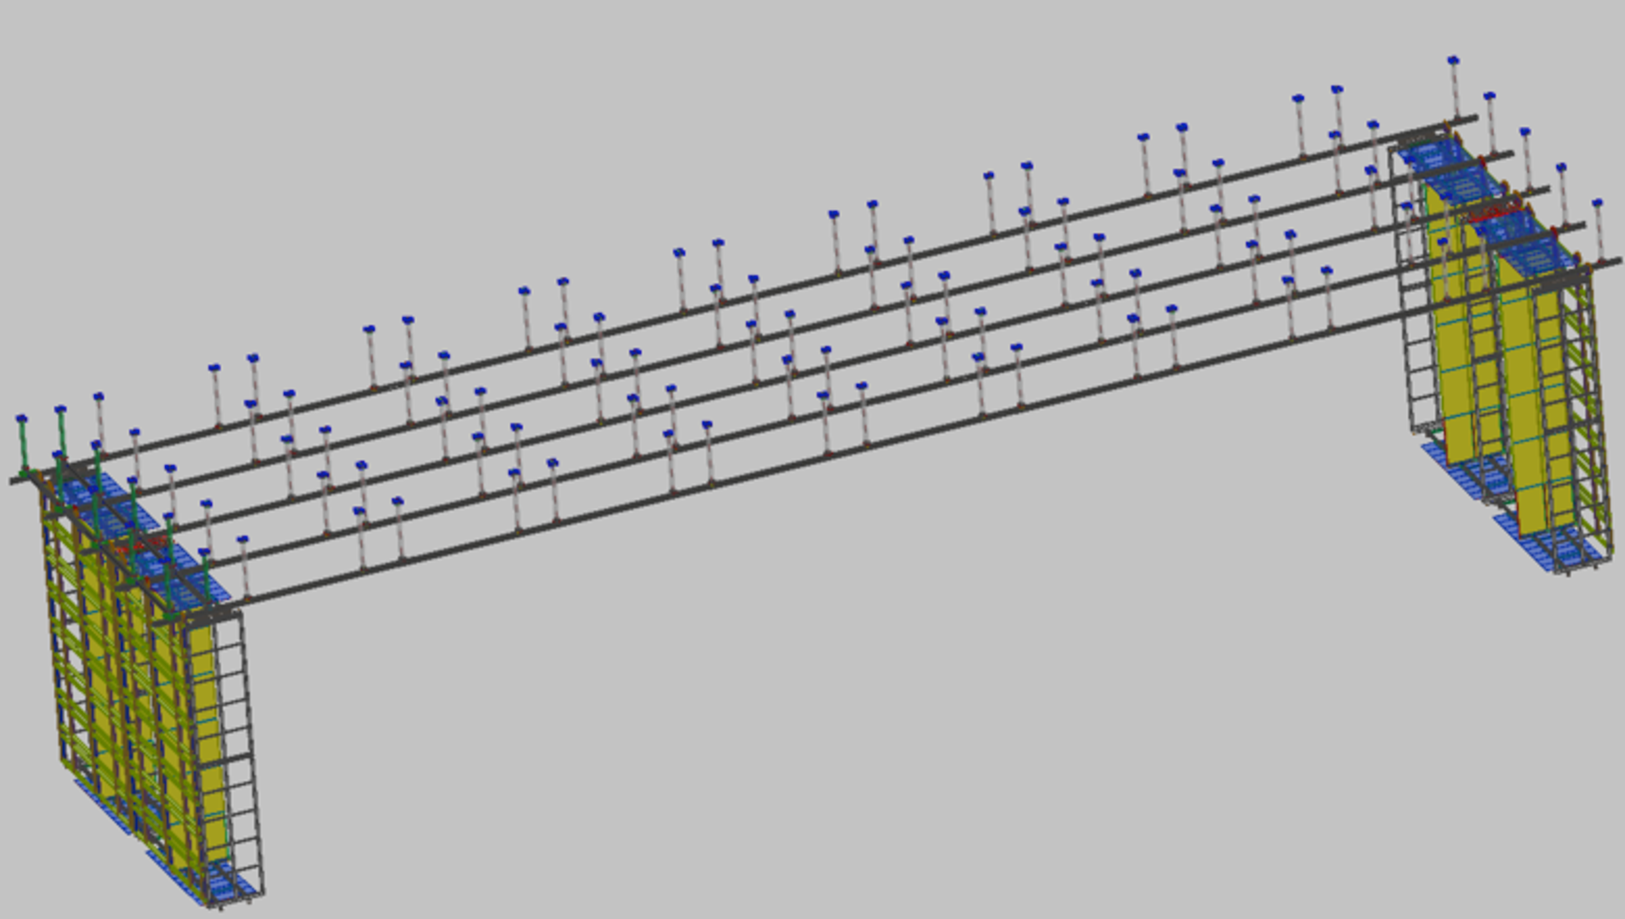
\includegraphics[width=.49\textwidth]{DSS-1.pdf}
 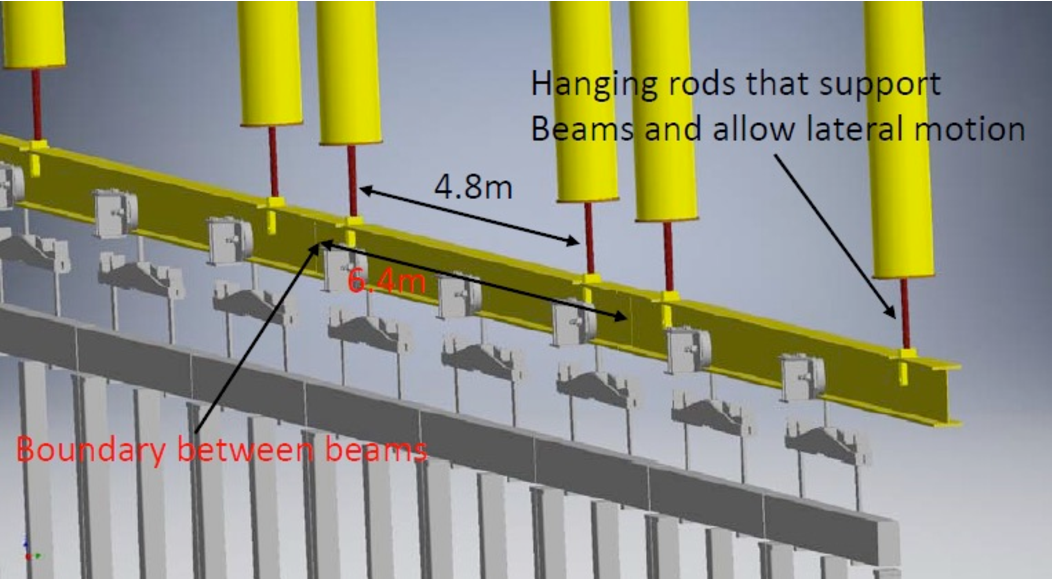
\includegraphics[width=.49\textwidth]{DSS-2.pdf}
\end{dunefigure}

The \dword{dss} is supported by the
cryostat outer steel structure through a series of \fdth{}s that cross through the cryostat insulation and anchored with flanges on
the cryostat roof. 
Inside the cryostat, a series of stainless steel I-beams are connected to the \fdth{}s and used to support the
detector. 
The \dword{dss} defines the location of the detector inside the cryostat and also defines how the detector elements move and contract as the detector is brought to \dword{lar} temperature. 
The design of the \dword{dss} encompasses the overall
structural design of the \dword{detmodule} because only after the elements are mounted to the \dword{dss} and connected do they make a unified mechanical structure. 
Figure~\ref{fig:DSS} (left) shows the \dword{dss} structure; there are
five rows of supports for the alternating rows of
\dword{apa}-\dword{cpa}-\dword{apa}-\dword{cpa}-\dword{apa}.  
The \dword{dss} is connected to the cryostat warm structure at a flange mounted on the outside of the cryostat.  
Figure~\ref{fig:DSS} (right)
shows the layout of these structural \fdth{}s.

The \dword{dss} is designed to meet the following  requirements:
\begin{itemize}
 \setlength\itemsep{1mm}
\setlength{\parsep}{1mm}
\setlength{\itemsep}{-5mm}
% \small
\item Support the weight of the detector;
\item Accommodate cryostat roof movement during filling, testing, and operation;
\item Accommodate variation in \fdth locations and
  variation in the flange angles due to installation tolerances and
  loading on the warm structure;
\item Accommodate shrinkage of the detector and \dword{dss} from ambient
  temperature to \dword{lar} temperature;
\item Define the positions of the detector components relative to each other; 
\item Provide electrical connection to the cryostat ground and remain electrically isolated from the detector;
\item Allow support penetrations to be purged with gaseous argon to prevent contaminants from diffusing back into the liquid; 
\item Ensure that the instrumentation cabling does not interfere with the \dword{dss};
\item Consist entirely of components that can  
be installed through the \dword{tco};
\item %Design to m
Meet AISC-360 or appropriate codes required at \dword{surf};
\item %Design to m
Meet seismic requirements one mile underground at \dword{surf};
\item Consist entirely of %All materials must be 
materials compatible for operation in ultrapure \dword{lar};
\item Ensure that beams are completely submerged in \dword{lar};
\item Ensure that detector components are not less than \SI{400}{mm} from the membrane flat surface;
\item Ensure that the supports do not interfere with the cryostat I-beam structures;
\item Ensure %Design such 
that the detector's lower \dword{gp} is lies over the cryogenic piping and that the tops of the \dword{dss} beams are submerged in \dword{lar} while leaving a \SI{4}{\%} ullage at the top of the cryostat;
\item Include the infrastructure necessary to move the \dword{apa} and
  \dword{cpa}-\dword{fc} assemblies from outside the cryostat through the
  \dword{tco} and to the correct position.
\end{itemize}

  The \dword{dss}
consists of pairs of \fdth{}s that support \SI{6.4}{m}-long
W10x26 stainless steel I-beam sections. The proposed design of the
\dword{dss} has \num{10} I-beam segments per row for a total of
\num{50} I-beam segments. Each I-beam is suspended on both ends by
rods from \fdth{}s that penetrate the cryostat roof.  %In the cold condition
When cold, each I-beam shrinks, causing gaps to form between
\dword{apa}s that are adjacent but supported on separate beams.
\dword{apa}s that are supported on the same beam will not have gaps
develop because both the beam and \dword{apa}s are stainless steel so
they shrink together.  Each beam is supported by a nearly
\SI{2}{m} long rod that allows the beam support to move as the beam
contracts.


The feedthrough consists of a flange and $6 ^{''}$ OD structural tube welded to it that extends through the cryostat insulation.  
There is a
nominal \SI{10}{mm} gap between the OD of the tube and the ID of the clearance tube in the cryostat. \fixme{OD and ID are not defined in the common glossary.}
The $6 ^{''}$ tube provides lateral support to the I-beams during installation.
Running down the center of the feedthrough is a $1^{"}$ diameter rod supported at a swivel washer at the flange and then supported by the
I-beam at a clevis.  The gas seal is obtained by Conflat Flange and a
bellows that seals around the swivel washer.  The lateral position and height of the rod can be adjusted $\pm$1 inch to accommodate tolerances in positioning cryostat crossing tubes. Figure \ref{fig:DSS-lateral-support} shows the end of the $6 ^{''}$ tube and how it locks the I-Beam into position. 

\begin{dunefigure}[DSS support for lateral loads ]{fig:DSS-lateral-support}
  {Left panel shows how the central support rod is locked in postion during detector installation. The outer $6 ^{''}$ tube is used to fix the support clevis in position. The right panel shows the system as it is connected to the I-Beam.}
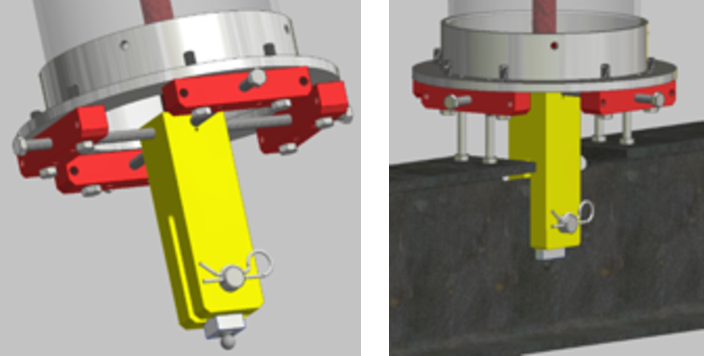
\includegraphics[width=.75\textwidth]{graphics/dss-lateral-support.pdf}
\end{dunefigure}

After the detector has been installed all restraints will be released to allow motion as the detector contracts during cool down.  The two hangars that support each \dword{dss} beam will contract and move toward each other by 13.1 mm along the axis of the detector.  
The drift distance will shrink by 7.4mm caused by the contraction of the field cages.  The detector is symmetric in the drift direction around the center \dword{apa}.  The drifts on either side of the center \dword{apa} will  shrink toward the center while the center \dword{apa} remains unmoved.  This results in the \dwords{cpa} moving 7.4mm toward the center and the outer \dword{apa}s moving 14.8mm (2*7.4mm) toward the center.  The hanging rod is designed to have a range of motion of 15mm in the drift direction to accommodate this shrinkage.




Detector components are installed using a shuttle beam system as
illustrated in Figure~\ref{fig:shuttle}.  
The last two columns of
\fdth{}s (eastern-most) support temporary beams that run
north-south, perpendicular to the main \dword{dss} beams.  
A shuttle beam has trolleys mounted to it and transverses 
north-south until it aligns with the required row of \dword{dss} beams.  
The last \dword{apa} or \dword{cpa} in a row is supported by the shuttle beam, which is bolted directly to the \fdth{}s once it is in place.  
As the last \dword{cpa} or \dword{apa} in each row is installed, the north-south beams are removed.

\begin{dunefigure}[\threed models of the shuttle beam end of the \dword{dss}]{fig:shuttle}
  {\threed models of the shuttle beam end of the \dword{dss}. The figures show how an \dword{apa}
is translated into position using the north-south beams until it lines up with the correct
row of I-beams.}
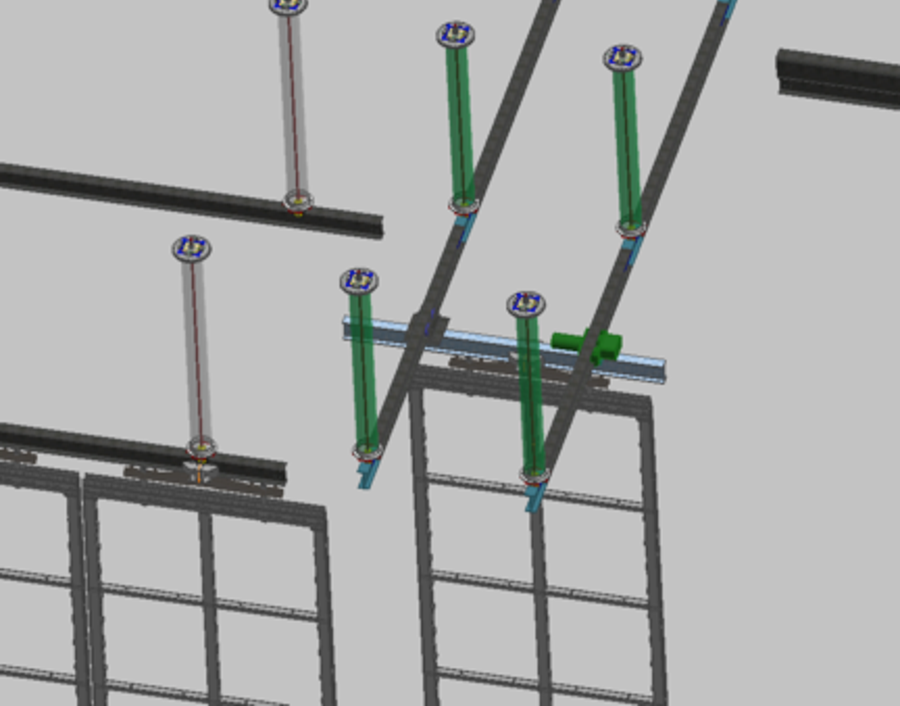
\includegraphics[width=.49\textwidth]{/Shuttle-1.pdf}
 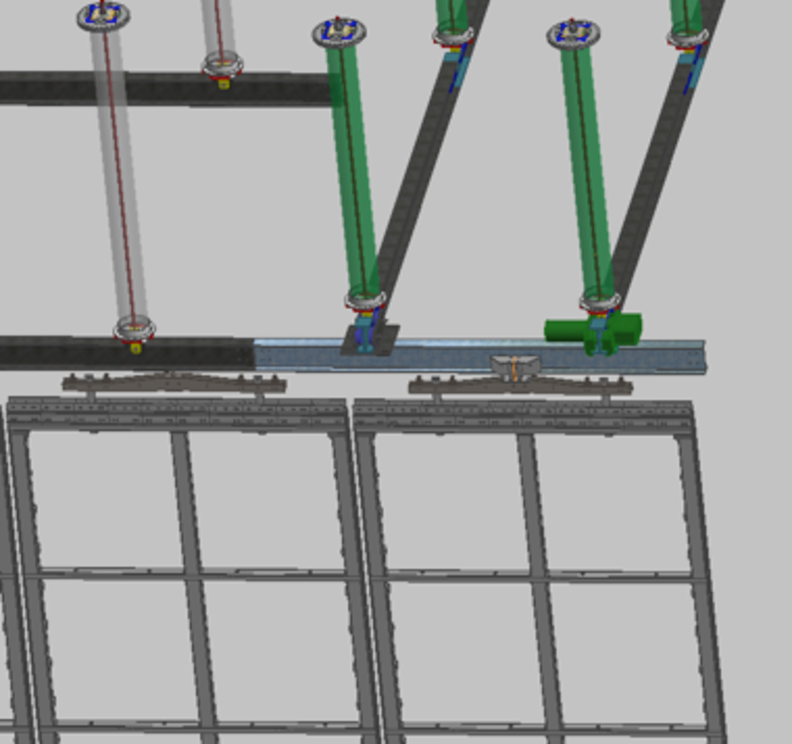
\includegraphics[width=.42\textwidth]{shuttle-2.pdf}
\end{dunefigure}

A mechanical interlock system  prevents trolleys
from passing the end of the shuttle beam unless it is aligned with a
corresponding \dword{dss} beam.  The shuttle beam and each detector component are
moved using a motorized trolley.  A commercially available motorized
trolley will be modified as needed for the
installation. 




\begin{dunefigure}[Prototype of the motorized DSS trolley ]{fig:DSS-trolley}
  {Prototype of the motorized DSS trolley that will push the APA and CPA along the I-beams and through the switchyard.}
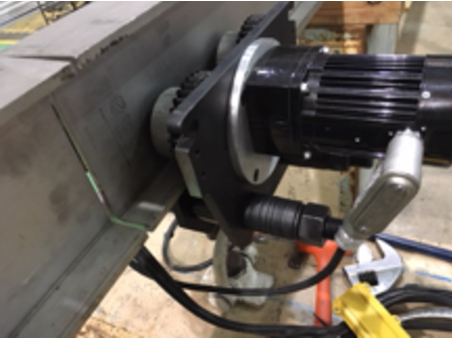
\includegraphics[width=.49\textwidth]{graphics/DSS-trolley.pdf}
\end{dunefigure}



A mock-up of the shuttle system will be constructed to test the
mechanical interlock and drive systems for the shuttle beam
for each \dword{detmodule}.  Tests will be conducted to evaluate the level of
misalignment between beams that can be tolerated and the amount of
positional control that can be achieved with the motorized trolley. We plan to construct a full scale prototype of a section of the  switchyard and perform tests at floor level. Later, the test program will be expanded at Ash River, where a full scale installation test will be performed. This is described in the installation \dword{qa} section.


%%%%%%%%%%%%%%%%%%%%%%%%%%%%
\subsection{Cryostat Roof Infrastructure}
\label{sec:fdsp-tc-infr-cryo-roof}



\begin{dunefigure}[Mezzanine and electronics racks]{fig:mezzanine}
  {The electronics racks sit on the \dword{dune} electronics mezzanine as shown. The top image is a view from above the detector looking at the racks from the side. In this view the cavern and cryogenics mezzanine are hidden. The bottom view is from the end of the cryostat looking over the roof. Here, the access stairs to the mezzanine are shown.}
 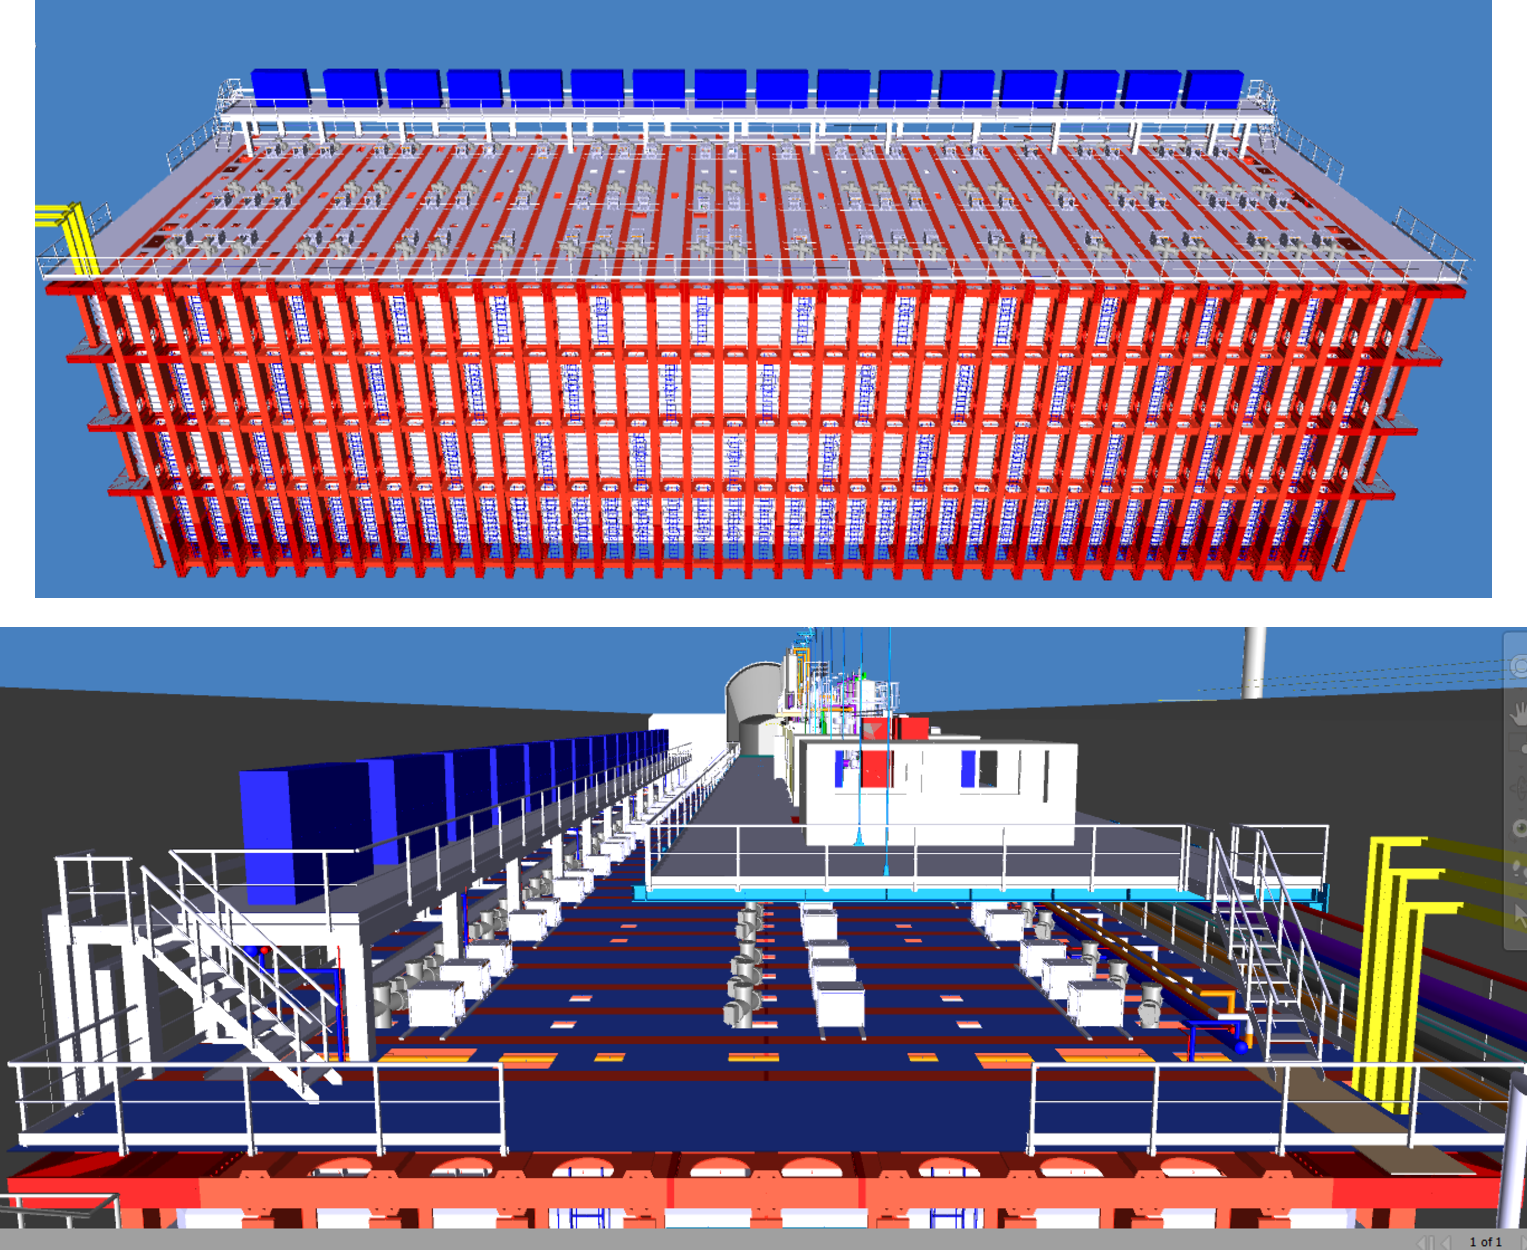
\includegraphics[width=\textwidth]{mezzanine.pdf}
\end{dunefigure}

\begin{dunefigure}[Electronics rack contents]{fig:rack-build1}
  {The nominal contents of the electronics racks on the mezzanine is shown. Each rack is configured to consume less than 3.5 \si{kW}. }
 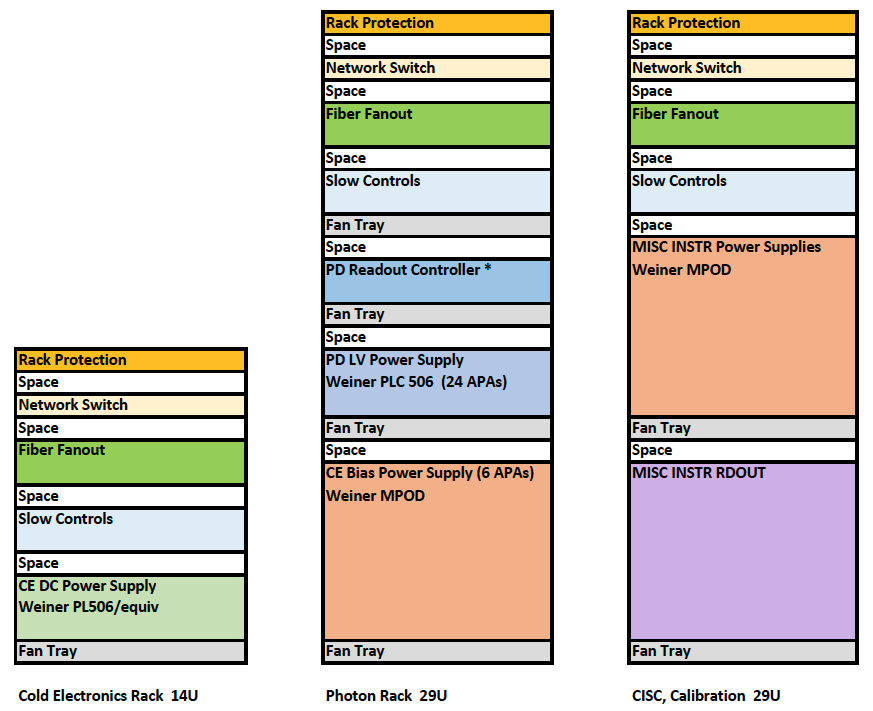
\includegraphics[width=.8\textwidth]{graphics/rack-build1.png} %pdf} It had too much room around it (was at .98)
\end{dunefigure}

The top image in Figure \ref{fig:mezzanine} shows the \dword{dune} electronics mezzanine with the 42U racks placed on top. 
\fixme{42U defined somewhere?} 
During the initial design steps, it became clear that the constraints placed on the rack location by the many \dword{dss} support feedthroughs, the electronics feedthrough, and the I-beams themselves make distributing the racks on the roof very challenging. 
By constructing a fixed mezzanine for the electronics 
above the cryostat at the same height as the cryogenic mezzanine, the electronics feedthroughs are kept clear. 
This configuration also makes working on the electronics much easier because there are no local obstacles and all the racks are in one place.

The racks are %on 
at detector ground, so the mezzanine, % is 
also at detector 
ground, % where it 
can simply be bolted to the cryostat I-beams. 
%As 
Figure \ref{fig:mezzanine} (top) shows 16 groups of five racks each %are 
on the mezzanine for a total of 80 racks. 
The heat load inside the detector racks will %should 
dissipate through air flow generated by cooling fans.  The major heat load resides with the cold electronics and photon electronics located near the cryostat feedthroughs.  If rack-mounted fans do not provide sufficient cooling,  \dword{cf} will provide sufficient water cooling capacity at the entrance to the North Cavern to accommodate the maximum heat load. 

%Twenty-five racks will be needed for cold electronics low voltage power and twenty-five racks are available for \dword{apa} wire bias voltage, \dword{pd} power and miscellaneous additional cold electronics, \dword{pd}, and  \dword{apa} electroncis modules. The remaining 30 racks will be available for slow control, calibration, and other miscellaneous electrical equipment. Small 12U high mini-racks will also be placed near the electronics feedthroughs for the \dword{pd} readout electronics and optical patch panels. If this is not enough, then additional racks can be placed on the cryostat roof. The present rack build for this layout is shown in Figure \ref{fig:rack-build1}. The modules inside the racks are distributed to keep power consumption for each rack below 3.5 \si{kW}.The racks to be installed will be 42U high, so we will have significant extra rack space.  If added electronics are needed for the \dword{ce}, however, we would need to install the modules in a \dword{pd} rack to stay under the power limit per rack.

Of the 80 racks, \dword{ce} \dword{lv} power require \num{25}, and another 25 will be made available collectively for  \dword{apa} wire bias voltage, \dword{pd} power and miscellaneous additional \dword{ce}, \dword{pds}, and  \dword{apa} electronics modules. The remaining 30 will be available for slow control, calibration, and other electrical equipment. Small 12U high mini-racks will  be placed near the electronics feedthroughs for the \dword{pd} readout electronics and optical patch panels. If this is not enough, additional racks can be placed on the cryostat roof. The present rack build for this layout is shown in Figure~\ref{fig:rack-build1}. 
\fixme{is `rack build' a common term? I would use `configuration'. anne} The modules \fixme{modules is used for so many things - can we use `items' here?} inside the racks are distributed to keep power consumption for each rack below \SI{3.5}{kW}.The racks are 42U high, which provides significant extra rack space.  If the \dword{ce} requires additional electronics, however, the items would need to go in a \dword{pd} rack to respect the per-rack power limit.

The 12U high mini-racks near the feedthrough flanges will be relatively empty because the \dword{pd} readout should need only approximately 2U in height while the \dword{ce} patch panel needs less than 1 U. The mini-racks are shown in the lower panel of Figure \ref{fig:mezzanine}; %fig:rack-build1}; 
they are the gray rectangles near the electronics crosses.

The north-south cable trays \fixme{where is north-south defined relative to the cryostats?  Can we add ``transverse to the beam?} running from the electronics mezzanine to the electronics feedthrough are routed under the floor of the cryostat roof next to the %cryostat 
I-beams. This keeps the roof reasonably clear, so that equipment can be transported across it. %the cryostat roof as needed. 
The gap between the web of the I-beams is \SI{1.2}{m}, such that % a 
installation of a \SIrange{200}{300}{mm} wide cable tray %can be installed while still leaving 
leaves enough space %to stand on the roof and 
for people to work on the electronics crates. 
The cable trays between the \dword{cuc} and the electronics mezzanine will run along the west end of the cryostat under the floor.  \fixme{which floor?}
We estimate only half of the \SI{1.6}{m} space is needed, so the cable tray quantity could in principal be doubled if necessary. 

The flooring material for the \dword{spmod} %should 
will be similar to the \SI{25}{mm} thick plywood used at \dword{pdsp}. %; it will be used for the final \dword{dune} detector. The flooring material 
It must be easy to cut so as to fit around many obstacles and pipes on the roof, it must be light enough to lift up to allow access under the floor, and it must support the load of a person %or 
and a small cart. 
We will investigate %what type 
fire-retardant options available %exist 
in the USA, %and will solicit 
with input the \dword{fnal} fire life-safety group. 

Air filters for the cleanroom and inside the cryostat will also be placed on the cryostat roof. The present plan is to place fan filter units near the manholes on the east end of the cryostat. Initial calculations indicate sufficient airflow is possible to support one air exchange per hour inside the cryostat. The air handling system has yet to be designed in detail.


\begin{dunefigure}[Cryostat crossing tube design]{fig:crossingtube}
  {Draft drawing of the cryostat crossing tubes. The hatched region is the cryostat insulation.}
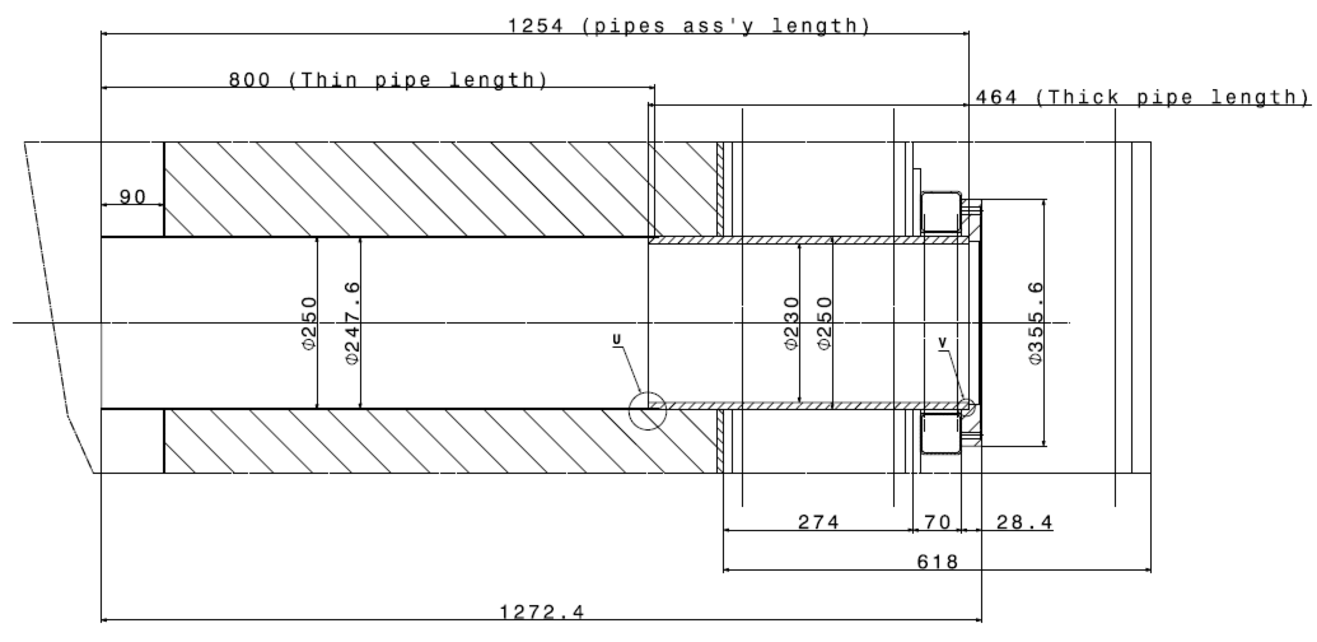
\includegraphics[width=.85\textwidth]{crossingtube}
\end{dunefigure}
\fixme{In figure \ref{fig:crossingtube} say what units are. mm? What are u and v? Clarify!}
 
The cryostat crossing tubes are among the most critical \fixme{challenging? Everything is critical, no?} components of the roof infrastructure. %These are the vacuum components that penetrate the cryostat roof and connect to the cold cryostat membrane. 
These  vacuum components penetrate the cryostat roof and connect to the cold cryostat membrane.The top flange of the crossing tube supports \fixme{either?} the electronics feedthrough or the detector support flanges and must be directly tied to the steel I-beams for support. %Accurately placing the crossing tubes and installing them true to vertical is important, ensuring the interface to the cryostat membrane can be made. 
Accurate placement and true vertical installation of the crossing tubes is important to ensure proper interfacing to the cryostat membrane. A draft assembly drawing of the crossing tube is shown in Figure \ref{fig:crossingtube}. The tube consists of a \SI{464}{mm} long stainless steel pipe with a \SI{1}{cm} \fixme{thick? and cm or mm?} wall. One end of the thin stainless steel tube is welded to the cryostat membrane, %at one end of the tube 
and the other to custom conflat flanges. % are welded to the other end. 
The %1 \si{cm} thick 
tube is welded to the steel roof plates.  \fixme{The cylindrical surface? which part?}


%To ensure that the crossing tubes are adequately cleaned during the initial gaseous argon (\dword{gar}) purge and that air is removed from the tubes, each crossing tube has a small side port connected to a network of pipes on the roof of the cryostat. During the initial \dword{gar} purge, argon gas is withdrawn from each port and analyzed to assess progress and determine when the system is ready to be cooled down. The large number of crossing tubes, about 250 in the \dword{sp} configuration, means the content from each port cannot be analyzed independently of all others. Five streams, each one collecting gas from about 50 crossing tubes are connected independently to the gas analyzers. Gas impurities accumulate in the ullage. During steady state operations, \dword{gar} from the crossing tubes will be analyzed to ensure that impurities are adequately removed from the \dword{gar}.    If additional cleaning of the ullage is necessary, the \dword{gar} withdrawn from all ports, or a smaller set of them, can be sent to the condenser, re-condensed, and purified in the liquid phase along with the rest of the \dword{lar}. To detect any possible leaks that could develop in the room temperature feedthroughs over time, simple O$^2$\ sensors monitor the return gas for traces of oxygen, which would indicate a leak.
 Each of the 250 crossing tubes has a small side port connected to a network of pipes on the roof of the cryostat. To ensure adequate cleaning and removal of air from the  tubes during the initial \dword{gar} purge,  \dword{gar} is withdrawn from each port and analyzed to assess progress and determine when the system is ready to be cooled down.  Five streams, each collecting gas from 50 crossing tubes, are connected independently to the gas analyzers. The collection and analysis of the gas will continue during steady state operations to ensure that impurities, which accumulate in the ullage,  are adequately removed from the \dword{gar}.    If additional cleaning of the ullage is necessary, the \dword{gar} from all or a subset of ports can be sent to the condenser, re-condensed, and purified along with the rest of the \dword{lar}. Simple O$_2$\ sensors monitor the return gas for traces of oxygen, which would indicate development of  a leak in the room temperature feedthroughs.

Each detector has a power budget of \SI{500}{kVA}. The total power budget available for use by detector electronics is derated to \SI{400}{kW} at the power distribution panels.  The \dword{ce} imposes the largest power load.  

The \dword{ce} dissipates \SI{306}{W} per \dword{apa}.  %The \dword{lv} power supplies have a controller that is about \SI{35}{W} per \dword{apa} and has an efficiency of approximately 85 percent.  
The \dword{lv} power supplies' controller imposes about \SI{35}{W} per \dword{apa} and has an efficiency of approximately 85 percent. This leads to an approximately  \SI{400}{W} load per \dword{apa}, or a total load of  \SI{60}{kW} per \dword{detmodule}.  The \dword{apa} wire-bias power supplies have a maximum load of  \SI{465}{W} per set of six \dword{apa}s, for a total budget of around  \SI{12}{kW}.   Cooling fans and heaters near the feedthroughs will use a nominal amount of power, so the overall power budget for \dword{ce} %should 
is expect to be less than \SI{75}{kW}.
\fixme{check my use of `imposes' vs `requires' vs `present' vs whatever for loads}

%The \dword{pds} electronics, based on the Mu2e electronics, report a power load of approximately 6KW.  A power budget of 8KW should be used because of cable drops and  power supply inefficiencies.  Please note that these \dword{pd} electronics are a significantly lower power load than the alternate \dword{protodune} solution of using \dword{ssp} modules at a power load of approximately 72 KW per detector.
The \dword{pds} electronics is based on the Mu2e electronics, which reports a power load of approximately  \SI{6}{kW}.  \dword{dune} plans a power budget of  \SI{8}{kW} because of cable drops and  power supply inefficiencies.  The \dword{pds} electronics present a significantly lower power load than the alternate solution, used in \dword{pdsp}, of using \dword{ssp} modules at a power load of approximately  \SI{72}{kW} per \dword{detmodule}.

Each of the approximately 80 detector racks will have fan units, Ethernet switches, rack protection, and slow controls modules, adding a load of about \SI{500}{W} per rack, for a total of \SI{40}{kW}.

%A number of racks are reserved for cryogenics instrumentation.  The load of these 25 racks is conservatively estimated at 2 KW per rack for a total of 50 KW.
Twenty-five racks are reserved for cryogenics instrumentation with a per-rack load conservatively estimated at \SI{2}{kW}, for a total of \SI{50}{kW}. 

The \dword{detmodule} will thus use  an estimated \SI{173}{kW} of power. The higher-load \dword{ssp} alternative for the \dword{pds} would increase this to \SI{237}{kW}.  These numbers provide a safety factor of about two on our power estimates relative to available power.


%%%%%%%%%%%%%%%%%%%%%%%%%%%%
\subsection{Cryostat Internal Infrastructure}
\label{sec:fdsp-tc-infr-cryo-int}


%%%%Internal Cryogenics%%%%
\label{sec:fdsp-tc-internal-cryo}

The internal cryogenics comprises three sets of pipe distribution networks and two sets of sprayers. All pipes enter the cryostat from the top; some go all the way down to the floor, and others remain in the ceiling. On the floor are
\begin{itemize}
\setlength\itemsep{1mm}
\setlength{\parsep}{1mm}
\setlength{\itemsep}{-5mm}
\item \textbf{GAr distribution}: a set of pipes flowing GAr. These pipes are used only at the beginning to remove air that fills the cryostat. They have either a longitudinal slit or calibrated holes to distribute GAr uniformly along the length of the cryostat. Computational fluid dynamics simulations show that air will be removed from the system as long as GAr is flowing in at the right speed, calculated and experimentally verified as \SI{1.2}{m/hr}.


\item \textbf{\dword{lar} distribution}: two sets of pipes flowing \dword{lar}. These pipes are used to fill the cryostat and, during steady state operations, to return the \dword{lar} from the purification system. The pipes have calibrated holes to return the \dword{lar} uniformly throughout the length of the cryostat. This is very important for uniform purity. Four pumps circulate the \dword{lar}. Initially, all of pumps operate at once to achieve purity, but once the target purity is achieved, only one or two pumps remain in service. Two sets of pipes are needed to adequately distribute the \dword{lar} over this broad range of flow rates.
\end{itemize}

On the ceiling are

\begin{itemize}
\setlength\itemsep{1mm}
\setlength{\parsep}{1mm}
\setlength{\itemsep}{-5mm}
\item \textbf{Cool down sprayers}: Two sets of cool down sprayers are distributed along the long sides of each cryostat. One set distributes \dword{lar} using liquid sprayers that generate a conical profile of small droplets of liquid. The other set of sprayers distributes GAr to move the \dword{lar} droplets inside and cool down the detector and cryostat uniformly. These sprayers are being tested in \dword{pddp}. They are a variation of those implemented in \dword{pdsp}.
\end{itemize}

Figure~\ref{fig:internal-cryo-3D} shows the current layout of the internal cryogenics. 
%The current drawing of the internal cryogenics is presented in Figure~\ref{fig:internal-cryo-drawing}. 
The GAr pipes are in red, the \dword{lar} pipes in blue.

\begin{dunefigure}[Cryogenic piping inside the cryostat ]{fig:internal-cryo-3D}
  {Layout of the internal cryogenics.}
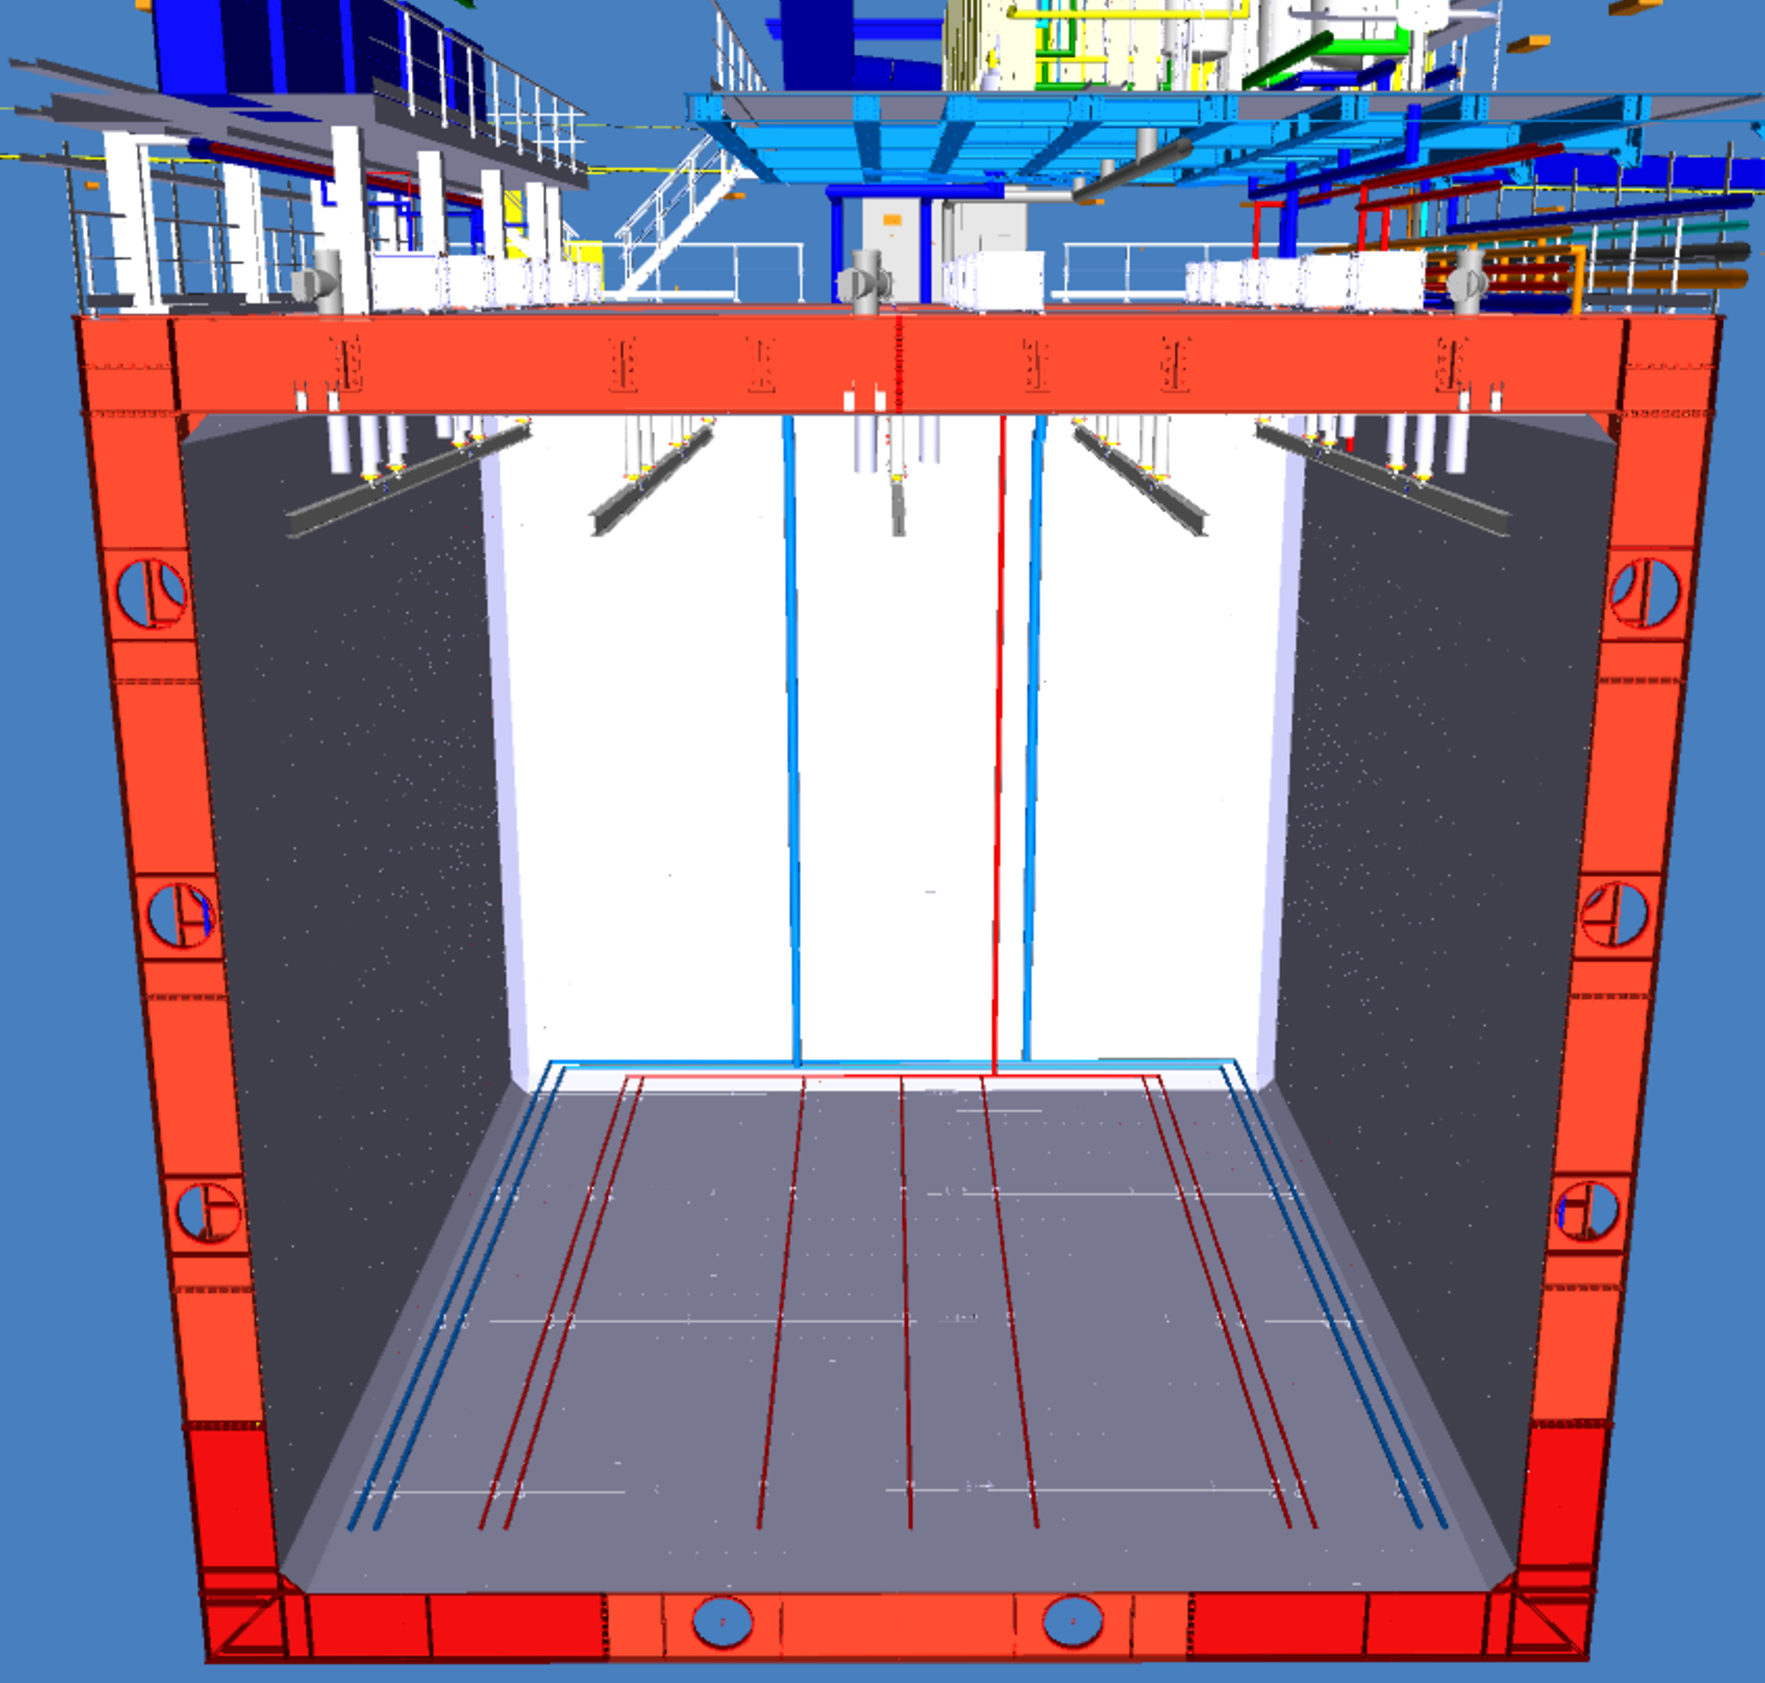
\includegraphics[width=.98\textwidth]{graphics/Internal-Piping-3D.pdf}
\end{dunefigure}

%\begin{dunefigure}[Drawing of the cryogenic %piping inside the cryostat %]{fig:internal-cryo-drawing}
%  {Drawing of the internal cryogenics.}
%\includegraphics[angle=90,width=.98\textwidth]{%graphics/Internal-pipes-HQ.pdf}
%\includegraphics[angle=90,height=.98\textheight%]{graphics/Internal-pipes-HQ.pdf}
%\end{dunefigure}
%\fixme{Please reduce size of Internal-pipes-HQ.pdf}


Other infrastructure inside the cryostat includes the cryostat false floor, the UV filtered lighting, and the battery-operated scissor lifts. 

The false floor %s not yet designed because the 
requirements are not yet fully defined. %The false floor 
It must support the load of the scissor lift used to work on the electronic cabling on the inside of the cryostat roof and allow the scissor lift to get close enough to the \dword{apa}s to work comfortably at the top. 
It  must be laid out so the panels can be removed in sections just before the equipment is installed,  %The space between the lowest point of 
except for the \dword{apa}s;  there is not enough room between the bottom of the \dword{apa}s %modules 
and the floor to allow removal. %is too small to allow the flooring to be removed once the \dword{apa} is in place. %However, t
%The floor panels in front of the \dword{apa} must % %Careful layout will be needed. 

The cryostat lighting, using UV-filtered \dword{led} lamps, is expected to be fairly simple. Options for the lighting will be developed during the Ash River testing. Floor-mounted lights with task lighting will be investigated. If needed, lighting can also be mounted to the \dword{dss} and removed as the detector is installed.

The plan is to use a commercially available battery-operated scissor lift with a 12 \si{m} reach. Tests at Ash River will verify the stability of the lift at the 12 \si{m} height. If the lift is determined to be suitable, then the remaining issue to resolve is how to install and remove it from the cryostat. The commercially available scissor lifts are too wide to fit through the \dword{tco} near the floor where the center post protrudes above floor level. Custom lifting equipment will be needed to insert the lifts into the cryostat. At the end of the installation process, dismantling the last lift may be necessary to remove it from the cryostat.

% clear the figure buffer before starting the next section
\clearpage

%%%%%%%%%%%%%%%%%%%%%%%%%%%%
\subsection{Cleanroom Infrastructure}
\label{sec:fdsp-tc-infr-comm}

\begin{dunefigure}[Installation Cleanroom layout]{fig:cleanroom-layout}
  {Two views of the installation cleanroom. The walls are shown as semi-transparent so the equipment inside can be seen. The left view is from the west looking east and shows the materials airlock (orange outline) and changing room (yellow outline). The cleanroom proper is behind the them and the cryostat is at the back. The second image on the right is a view looking north. It shows the outline of the cleanroom in green. The cryostat is on the left of the cleanroom and the airlocks on the right.} 
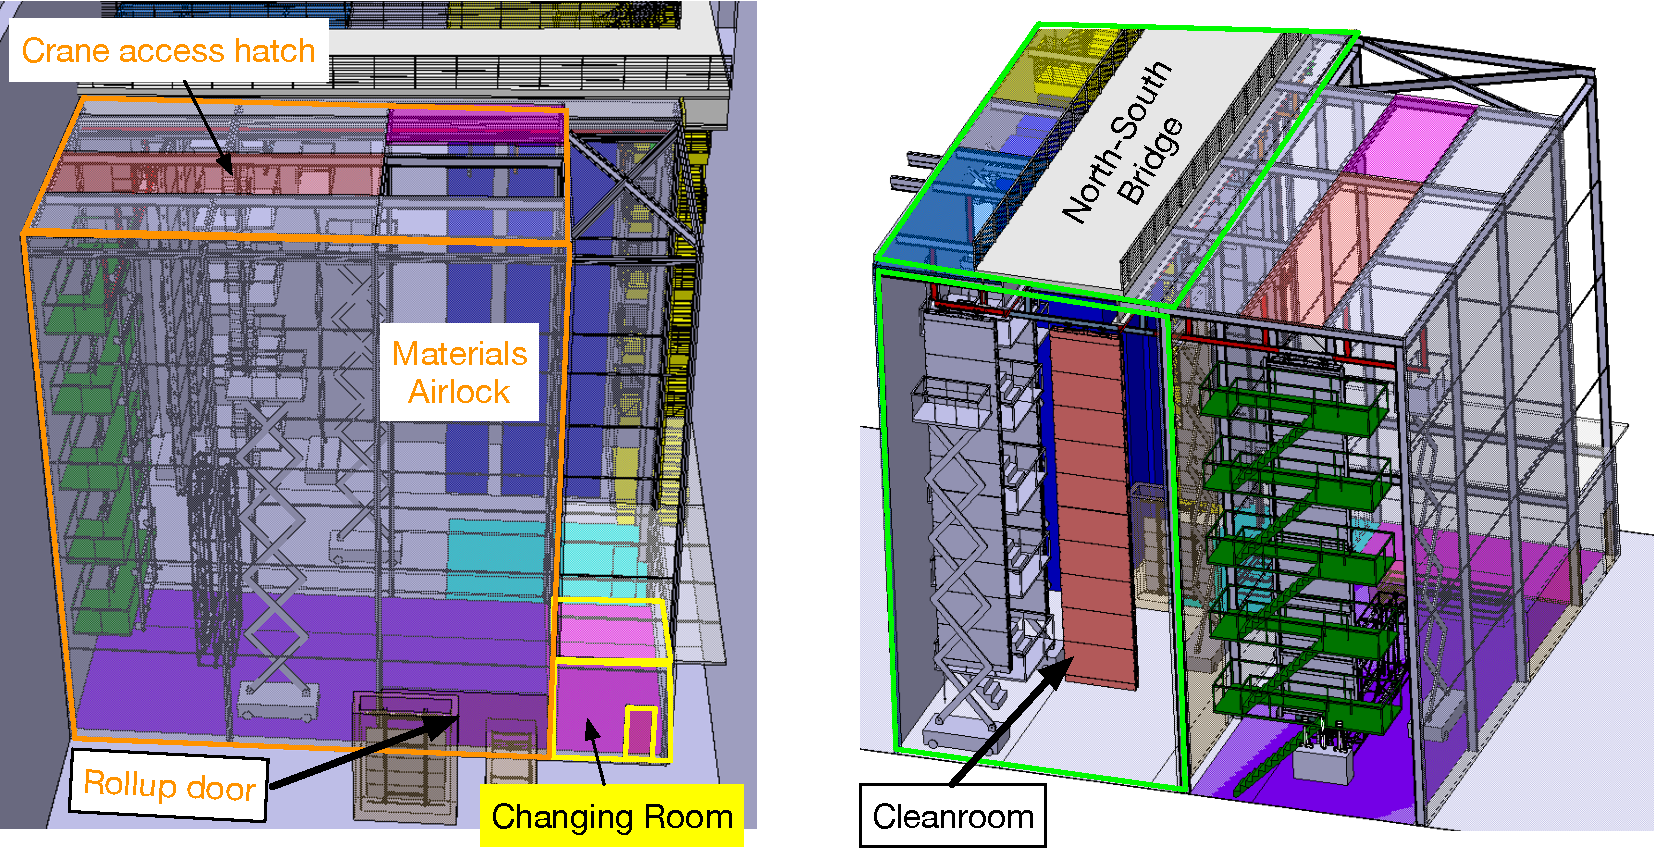
\includegraphics[width=1.0\textwidth]{cleanroom-layout}
\end{dunefigure}
\fixme{for fig \ref{fig:cleanroom-layout}: walls are semi-transparent IN THE FIGURE, not for real ( I added `shown as'). Directions are confusing -left, right, west, north.  Also would be nice to add a person to show scale.}

The assembly of the detector sub-components into \SI{12}{m} tall full assemblies %modules 
must be done underground directly outside the cryostat. The full %12 \si{m} long 
assemblies are too large and fragile to be brought down the shaft, and the only place with enough vertical space to assemble them is in front of the cryostat itself. A combination of contractors and the lead worker and rigger teams will do the infrastructure work; they will also assist in detector assembly. The cleanliness requirement for all work on the components inside the detector means that all work must be done in an ISO-8 cleanroom, so a very large cleanroom must be built outside the cryostat containing all the necessary infrastructure to assemble the %detector \dword{tpc} elements. 
\dword{lartpc} components. Figure \ref{fig:cleanroom-layout} illustrates %provides an image of 
the conceptual design of the installation cleanroom. The left figure is an end view of the cleanroom, showing the materials airlock 
\fixme{at the back (east end) ?} 
and the changing room. The right image is a side view showing the cleanroom on the left and the airlock on the right.

The plan is to bring all detector elements into the cleanroom through large roll up doors in the side wall of the airlock. The materials will be moved using using  a battery operated forklift and electric pallet jacks. The airlock will be  13 \si{m} wide 10 \si{m} deep and 17 \si{m} tall. This is large enough to hold the \dword{apa} assembly tower described below with enough extra space to move large objects inside. An access hatch is planned for the roof, allowing the cavern bridge crane to be used in the central area of the airlock. The crane is needed to manipulate the \dword{apa} modules in the airlock; the plan calls for assembly of the double-high \dword{apa} pairs there. Also shown on the right of the figure is the changing room for the cleanroom. The changing room is 3 \si{m} wide and 10 \si{m} deep. The dimensions were chosen to allow 20-30 people to gown up for the cleanroom within a reasonable time. The requirements for work in an ISO-8 cleanroom are a cleanroom lab coat, clean shoes, and nets for hair and beards.  This will be augmented with a clean hard hat and gloves for safety reasons. 

The outline of the cleanroom proper is shown on the right in Figure \ref{fig:cleanroom-layout}. The cleanroom dimensions are 16 \si{m} wide 10 \si{m} deep and 17 \si{m} tall. The cleanroom lies primarily under the north-south bridge and in the 3.4 m space between the bridge and the cryostat. %Here operations that must be performed are the 
Cabling of the \dword{apa}, cold testing of the \dword{apa}, and assembly of the cathode \dword{fc} modules will take place here. The tower for the \dword{apa} cabling, the \coldbox{}es for testing, and the switchyard for moving the 12m tall objects are described below. All areas of the airlock and cleanroom will be outfitted with UV filtered lights. In addition to this cleanroom, the inside of the cryostat will also be effectively a cleanroom.  By filtering the air and forcing it  into the cryostat at the east end, the clean air will flow through the cryostat and out through the cleanroom and airlock. This will keep the inside of the cryostat at least at ISO-8. The construction process for the cleanroom is still at the conceptual level so what is shown is a steel frame structure where panels can be mounted. %The size is substantial and the occupancy significant, so the cleanroom should have electrical outlets, UV filtered lighting, and fire protection. 
Given the substantial size and the significant occupancy, the cleanroom will have electrical outlets, UV filtered lighting, and fire protection. 

\fixme{need to check all dimensions and update the figure}

\begin{dunefigure}[APA assembly tower]{fig:apa-assemble-frame}
  {The \dword{apa} assembly tower with the \dword{apa} assembly frame attached. The transport rails at the top of the figure are used to move the assembled \dword{apa} into the cleanroom. The work decks allow access to the \dword{apa} from multiple levels. }
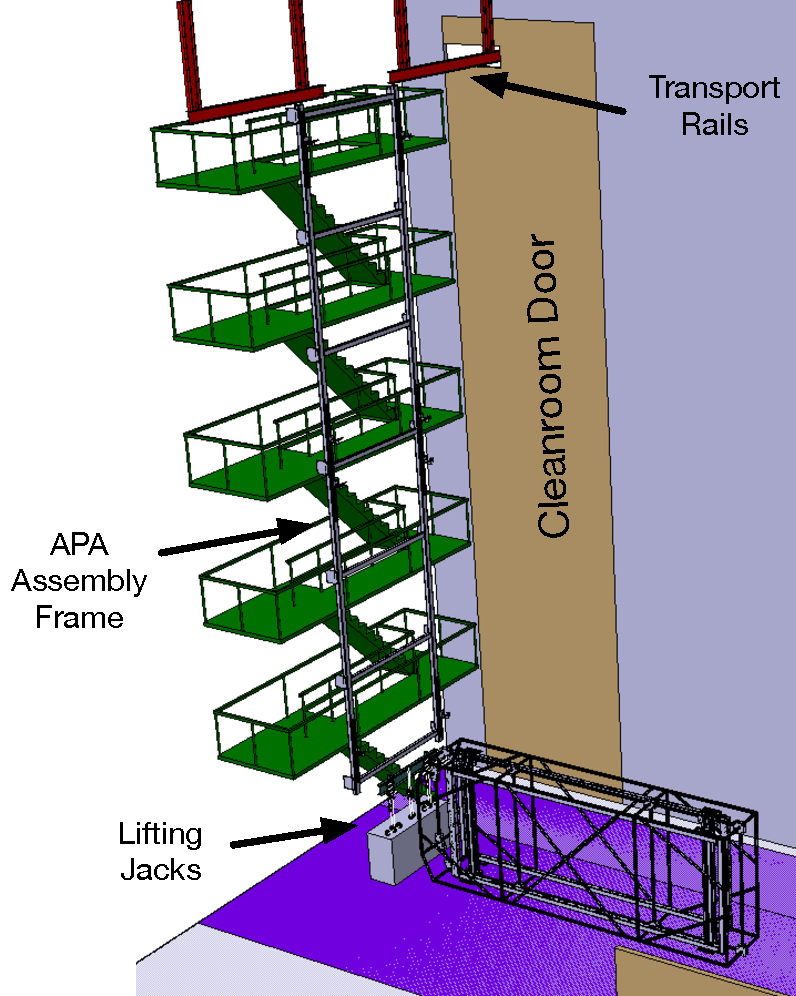
\includegraphics[width=.5\textwidth]{apa-assemble-frame}
\end{dunefigure}

\fixme{need to update the figure}

The \dword{apa} assembly tower is a six story tall stair tower used to assemble the individual \dword{apa} modules into the final 12 \si{m} tall pair. 
The tower is designed to so that the stair landings will allow access to the sides and top of the \dword{apa} as required for assembly. 
The \dword{apa} assembly tower also provides support for the the \dword{apa} assembly fixture provided by the \dword{apa} consortia. 
The \dword{apa} assembly fixture is the tooling needed to hold the upper and lower \dword{apa} during assembly and to bring the two modules together so they can be connected. 

Figure \ref{fig:apa-assemble-frame} shows an image of the \dword{apa} assembly tower. 
In this figure, the \dword{apa} assembly frame is shown mounted on the assembly tower, and an \dword{apa} transport box is on the airlock floor in front of the tower. 
At the top of the \dword{apa} assembly tower is a set of I-beam rails used to move the \dword{apa} pair into the cleanroom through a sliding door shown in brown. 
The final trolleys will be used from this step forward. 
Care will be taken in the \dword{apa} assembly steps to remove only a minimal amount of the dust protection from the \dword{apa} because manipulating the \dword{apa} must be performed using the cavern bridge crane, which will require an opening in the roof. 
Once the \dword{apa}s are assembled, the bridge crane is no longer needed, and the roof opening is closed. Air is then circulated until the required purity is met. The tower shown in Figure \ref{fig:apa-assemble-frame} has landings that will meet safety codes, but the outer steel frame to support the landings has not yet been designed.


\begin{dunefigure}[APA cabling tower]{fig:apa-cable-tower}
  {The \dword{apa} cabling tower. The two reels of cable for the electronics are shown. The work decks allow access to the \dword{apa} from multiple levels. }
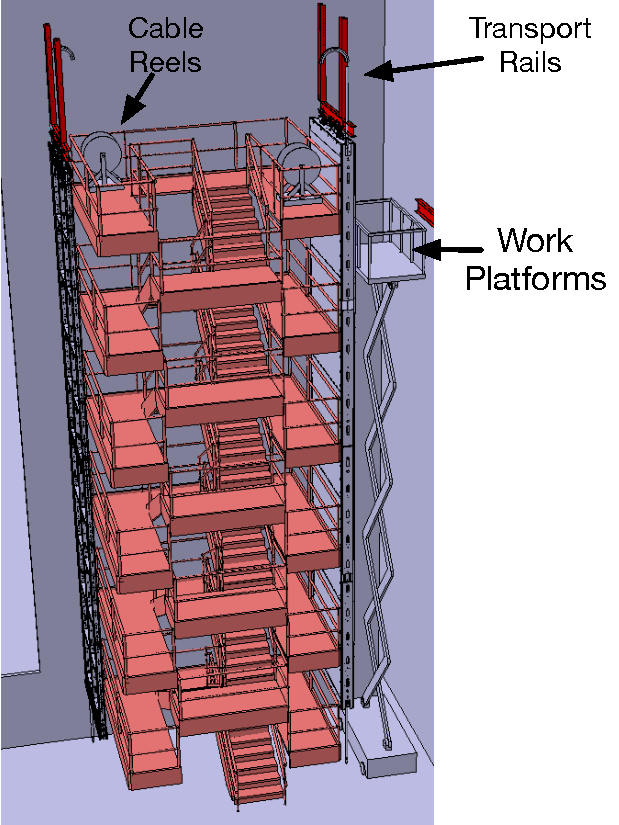
\includegraphics[width=.5\textwidth]{apa-cable-tower}
\end{dunefigure}

%Inside the cleanroom is another stair tower used for cabling and the initial tests of the \dword{ce}. 
Inside the cleanroom  another stair tower is used for cabling the \dword{apa}s and the initial tests of the \dword{ce}. Due to the time required for cabling and testing of the electronics in \dword{protodune}, % show that 
two workstations are needed. The \dword{apa} cabling tower is shown in Figure \ref{fig:apa-cable-tower}. The \dword{apa} cabling tower is a stair tower similar to the \dword{apa} assembly tower, where access is provided to the sides of the \dword{apa} at many levels, and a dedicated lift provides access on the outer face. The cable is brought up to the top of the platform on spools using the switchyard described below. The \dword{apa}s are moved next to the stair tower work faces, also using the switchyard.  Sufficient space is needed at the top levels to allow people to work on the cabling and test the electronics. The size and the layout of the top level of the tower will be optimized based on input from the future prototyping tests %to be done 
at Ash River. 

\begin{dunefigure}[Cleanroom material transport system]{fig:cleanroom-switchyard}
  {The switchyard inside the cleanroom and airlock. The beams of the switchyard are highlighted in red. Fixed beams running east to west (the \dword{detmodule}'s long axis) are used to move the The \dword{apa} and The \dword{cpa} to a dedicated work location while a bridge crane running north-south is used to transport the units between the different fixed beams. }
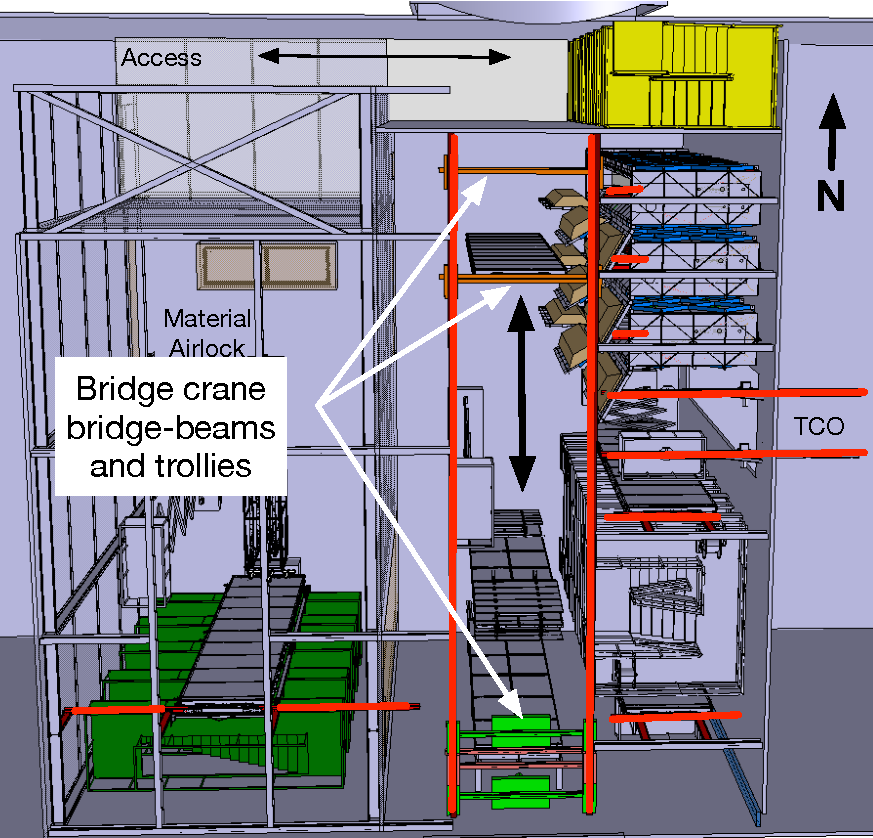
\includegraphics[width=.75\textwidth]{cleanroom-switchyard}
\end{dunefigure}

Once the \dword{apa} pair or the \dword{cpa} panels are assembled, the units will be moved around the cleanroom and airlock using a dedicated rail-based switchyard (I-beam and trolley). The switchyard is illustrated in Figure \ref{fig:cleanroom-switchyard}; %in the center of the figure is 
the bridge crane, which travels north-south, is in the center. Several bridge beams driven by electric trolleys %will 
move on the runway beams of the crane.  By aligning the bridge beams with a set of fixed beams supported from the cleanroom roof, the \dword{apa} and \dword{cpa} can be transferred from the fixed beams to the bridge crane and %then 
moved to different locations in the cleanroom. Figure~\ref{fig:cleanroom-switchyard} shows a single fixed beam in front of the \dword{apa} assembly tower in the airlock and seven locations on the right where equipment can be moved during assembly and testing. The work stations are on the two faces of the \dword{apa} cabling tower, the two beams through the \dword{tco} \fixme{are?} used to move the finished detector into the cryostat, and the three I-beams  \fixme{are?} used to move the \dword{apa} into the \coldbox{}es in the northeast corner of the cleanroom. An additional fixed beam must be added over the cabling tower to allow hoisting the cable reels %to be hoisted
to the top. 

%%%%%%%%%%%%%%%%%%%%%%%%%%%%
\subsection{Cryogenics and \coldbox{}es}
\label{sec:fdsp-tc-infr-cryo}

\fixme{anne to here 3/11}


After an \dword{apa} pair is fully assembled and cabled but before installation, it is thermally cycled  % before being installed in the cryostat. %To do this, three tall but narrow cryostats are needed that can be cooled as close to LAr temperature as reasonably possible. These cryostats are referred to as \coldbox{}es and require a dedicated cryogenics system. 
in a tall narrow cryostat, called a \coldbox{}, shown in Figure~\ref{fig:install-coldbox}). To test \dword{apa}s at a rate necessary to keep up with the installation plan, we will use three identical \coldbox{}es in the cleanroom. The \coldbox{}es require a dedicated cryogenics system that cools them  close to \dword{lar} temperature. 


%The \coldbox{}es used to thermally cycle the assembled \dword{apa} pairs before they are installed in the cryostat are shown in Figure~\ref{fig:install-coldbox}. To test \dword{apa}s at a rate necessary to keep up with the installation plan, three \coldbox{}es are needed inside the cleanroom. Each \coldbox has external dimensions of 14.0 \si{m} by 3.2 \si{m} by 1.3 \si{m} (H $\times$ L $\times$ W). Three layers of 100 \si{mm} thick foam insulation are used for the thermal isolation. This gives an internal dimensions of 13.4 \si{m} x 2.6 \si{m} x 0.7 \si{m} (H $\times$ L $\times$ W). Inside each \coldbox, a rail section similar to the ones used in the \dword{tco} as well as other fixed rails in the cleanroom will be mounted.This will allow the \dword{apa} to be pushed into the \coldbox{}es using the cleanroom switchyard and trolleys. A support base will be needed under the \coldbox{}es to adjust the height to mate with the cleanroom switchyard.

% Each \coldbox has external dimensions of 14.0 \si{m} by 3.2 \si{m} by 1.3 \si{m} (H $\times$ L $\times$ W). Three layers of 100 \si{mm} thick foam insulation are used for the thermal isolation. This gives an internal dimensions of 13.4 \si{m} x 2.6 \si{m} x 0.7 \si{m} (H $\times$ L $\times$ W). Inside each \coldbox, a rail section similar to the ones used in the \dword{tco} as well as other fixed rails in the cleanroom will be mounted.This will allow the \dword{apa} to be pushed into the \coldbox{}es using the cleanroom switchyard and trolleys. A support base will be needed under the \coldbox{}es to adjust the height to mate with the cleanroom switchyard.

A \coldbox has external dimensions of 14.0 \si{m} by 3.2 \si{m} by 1.3 \si{m} (H $\times$ L $\times$ W). With three layers of 100 \si{mm} thick foam insulation,  
the internal dimensions are 13.4 \si{m} by 2.6 \si{m} by 0.7 \si{m}. A rail section similar to those used elswhere in the cleanroom will be mounted inside each \coldbox to allow the cleanroom switchyard and trolleys to push an  \dword{apa}  into a \coldbox. A support base under the \coldbox{}es will adjust the height to mate with the cleanroom switchyard.

%The \coldbox{}es will have an electronics feedthrough similar to what is used on the top of the \dword{dune} cryostat, except that short cables will be run from the \dword{wec}  to a patch panel inside the \coldbox.This will allow the cable on the \dword{apa} to be connected directly to the test readout without having to remove any cabling. Each \coldbox will be designed like the successful \dword{protodune}-\dword{sp} \coldbox. The outer shell is constructed of a stainless steel plate with reinforcing ribs welded on. The biggest difference between the \dword{dune} \coldbox{}es and the \dword{protodune}-\dword{sp} \coldbox, other than doubling the height, is that a hinged door is planned for the \dword{dune} \coldbox{}es. In \dword{protodune}, unbolting the door and lifting it off the \coldbox required significant effort. In \dword{dune}, the cleanroom does not have full crane coverage, so doors that can be opened and closed using a scissor lift are necessary.Initial estimates are that the \dword{dune} \coldbox{}es will need about 11 \si{T} of stainless steel. They must be assembled in place because the finished boxes are too big to fit down the Ross Shaft. The \coldbox base must be on Hilman rollers, so the boxes can be moved under the bridge after installation to allow installation of the cryogenic circulation pumps.
 
The \coldbox electronics feedthroughs will be  similar to what is used on the top of the \dword{dune} cryostat, except that short cables will be run from the \dword{wec}  to a patch panel inside the \coldbox. This will allow the cable on the \dword{apa} to connect directly to the test readout without having to remove any cabling. The \coldbox  design is nearly the same as the successful \dword{pdsp} \coldbox. The outer shell is similarly constructed of a stainless steel plate with reinforcing ribs welded on. The height is of course doubled, and a hinged door is planned. Unbolting the door and lifting it off the \dword{pdsp} \coldbox required significant effort, and lacking full crane coverage in this case, doors that can be opened and closed using a scissor lift are necessary. The \dword{dune} \coldbox{}es will collectively need about 11 \si{T} of stainless steel, according to initial estimates. They must be assembled in place because the finished boxes are too big to fit down the Ross Shaft. The \coldbox base must be on Hilman rollers, so the boxes can be moved under the bridge after \fixme{detector?} installation  to allow installation of the cryogenic circulation pumps.




\begin{dunefigure}[Installation \coldbox]{fig:install-coldbox}
  {\coldbox{}es used to thermally cycle the fully assembled APA pairs. }
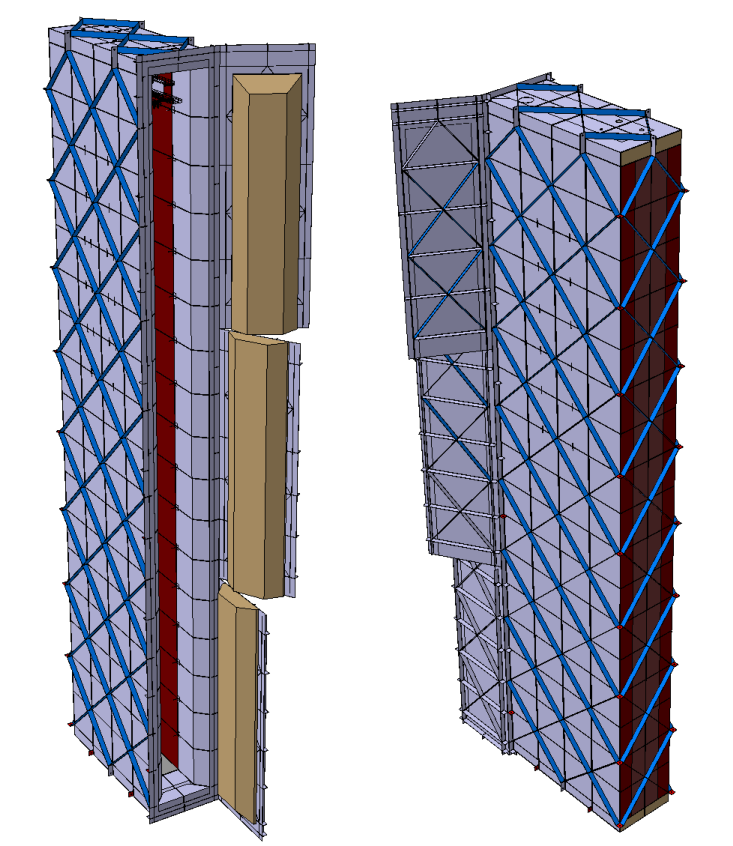
\includegraphics[width=.5\textwidth]{graphics/install-coldbox.pdf}
\end{dunefigure}

%DAVID added cryo cold box%%
%\subsubsection{Cryogenics supporting the Cold--Boxes}
%{Cold Boxes Cryogenics}
\label{sec:fdsp-tc-cryocoldbox}

%The cryogenics supporting the \coldbox{}es underground must ensure reliable and safe operation of the system used to test the \dwords{apa} that will be installed inside the cryostats. The main functional requirements of the system are
The  \coldbox{}es will be used to test the \dword{apa}s underground prior to installation. % in the cryostat. 
The cryogenics supporting the \coldbox{}es  must ensure their reliable and safe operation; to that end, it must
\begin{itemize}
\setlength\itemsep{1mm}
\setlength{\parsep}{1mm}
\setlength{\itemsep}{-5mm}
\item support three \coldbox{}es operating in parallel: %for testing dual \dword{apa}s: 
one in \cooldown mode, two either in steady-state or warm-up modes.
\item allow personnel in the cleanroom during all phases of the purge, \cooldown, operation, and warm-up modes. 
\item test the detector modules at near \dword{lar} temperature.
\item operate 24 hours a day, seven days a week for 10 years.
\item allow remote operations.
\item be located in the vicinity of the \dword{tco}. Space is available on top of the cryogenic mezzanine on the roof of the cryostat.
\end{itemize}

It must operate in the following modes: %fulfill the following modes of operations:

\begin{itemize}
\setlength\itemsep{1mm}
\setlength{\parsep}{1mm}
\setlength{\itemsep}{-5mm}
\item \textbf{purge}: During this mode, air is removed from the system (\coldbox and cryogenic system) and replaced with dry nitrogen. The concentration of moisture is monitored, and when it no longer decreases, the \cooldown can commence.
\item \textbf{\cooldown}: Cold nitrogen is introduced into the system to cool the inside of the \coldbox and the \dword{apa} inside it. %it down and to cool down the detector contained inside the coldbox. 
This should take 24 hours, during which time the temperature decreases from room temperature to about \SI{90}{K}. 
\item \textbf{steady-state operations}: After reaching %the nominal temperature of 
approximately \SI{90}{K}, %the value is maintained for 48 hours, during which 
the detector is turned on and fully tested. % at cold. 
This takes about 48 hours.
\item \textbf{warm-up}: After completing the test, the system is %slowly 
warmed up to room temperature over a period of 24 hours. %This should take 24 hours, during which the temperature goes from approximately \SI{90}{K} to room temperature.
\end{itemize}

\begin{dunetable}
[\Coldbox  cryogenics system parameters] %for specifications]
{lc}
{tab:table-cryo-coldboxes}
{Table of parameters for the \coldbox cryogenics system.}
Parameter & Value 
\\ \toprowrule
Dual \dword{apa} thermal mass &  1,600 kg\\ \colhline
Temperature uniformity & $+60$ K / $-0$ K \\ \colhline
Electronics load & 300 W \\ \colhline
\Coldbox insulation thickness &  0.3 m \\ \colhline
Target \cooldown temperature &  \SI{90}{K} \\ \colhline
Target \cooldown duration &  24 hr \\ \colhline
Target steady-state duration &  48 hr \\ \colhline
Target warm-up duration &  24 hr \\ \colhline
Maximum cooling power  &  \SI{13}{kW}  \\ \colhline 
Maximum liquid nitrogen consumption  &  \SI{300}{l/hr}  \\ \colhline 
\end{dunetable}

The evaporation of liquid nitrogen provides the cooling power for the system. Warm nitrogen and a heater provide the heating power. At peak consumption, the expected maximum heat load is \SI{8.5}{kW}. Assuming a 50\% margin on the refrigeration load, the cryogenics system requires \SI{13}{kW} of net cooling power at peak consumption, which equals about \SI{300}{l/hr} of evaporating liquid nitrogen.

Two layouts are currently under consideration: (1) a closed loop with mechanical refrigeration, in which liquid nitrogen is generated {\it in situ}, circulated, and the spent nitrogen recondensed before being put back into the system; and (2) open loop, in which liquid nitrogen is transported underground by means of portable dewars, circulated, and the spent nitrogen vented away. For the closed loop, we would need a mechanical refrigeration capable of supplying \SI{13}{kW} of cooling. For the open loop, it is possible to use a \SI{2000}{l} dewar, which is commercially available and transportable up and down the Ross Shaft inside the cage. To supply the required amount of nitrogen, four trips per day are needed.

The current versions of the closed loop and open loop systems are presented in Figures~\ref{fig:mechanical-refrigeration} and~\ref{fig:LN2}, respectively. % . The current version of the open loop system is presented in Figure~\ref{fig:LN2}.

\begin{dunefigure}[\Coldbox cryogenics support system based on mechanical refrigeration ]{fig:mechanical-refrigeration}
  {Layout of the cryogenics supporting the \dword{apa} test facility with mechanical refrigeration (closed loop).}
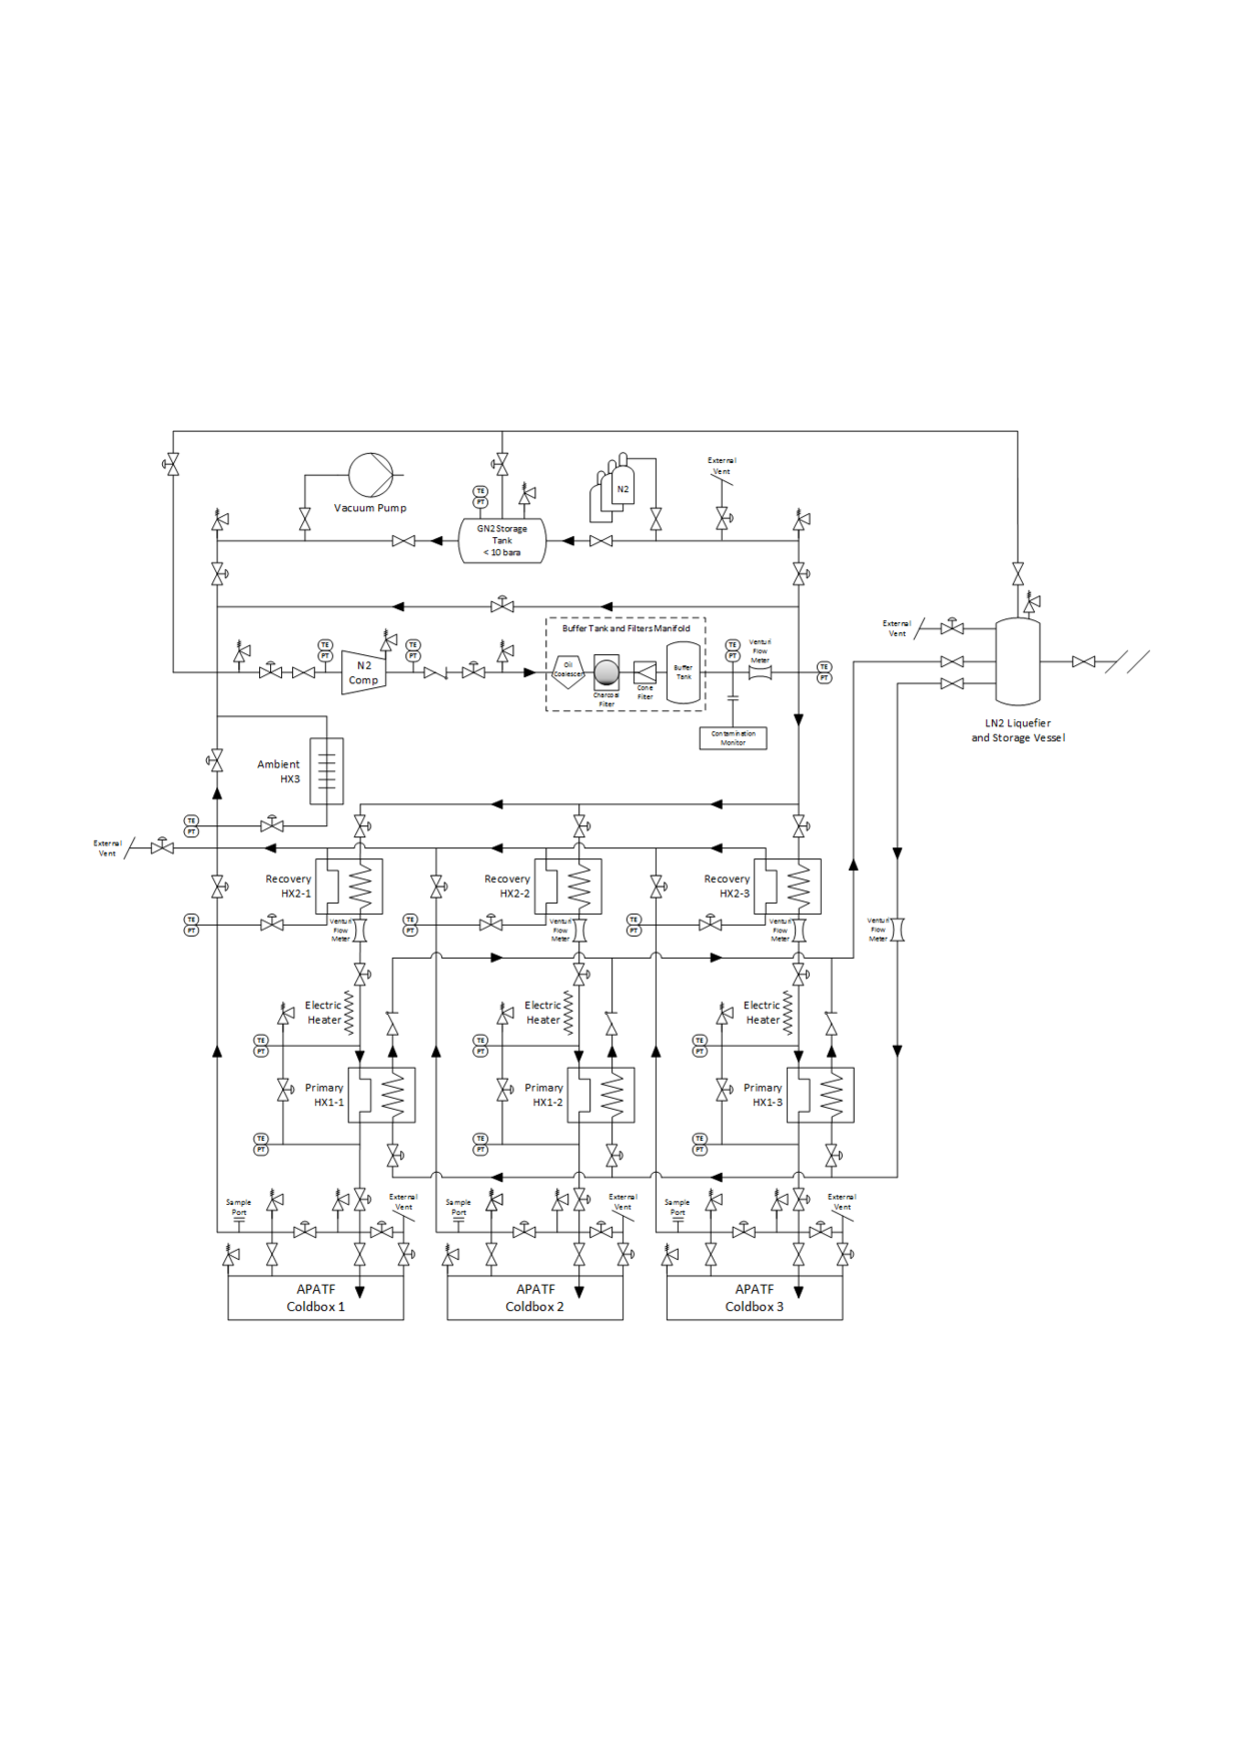
\includegraphics[width=.98\textwidth]{graphics/Cryo-cold-box-mechanical.pdf}
\end{dunefigure}

\begin{dunefigure}[\Coldbox cryogenics support system based on LN2 ]{fig:LN2}
  {Layout of the cryogenics supporting the \dword{apa} test facility with open loop refrigeration (open loop).}
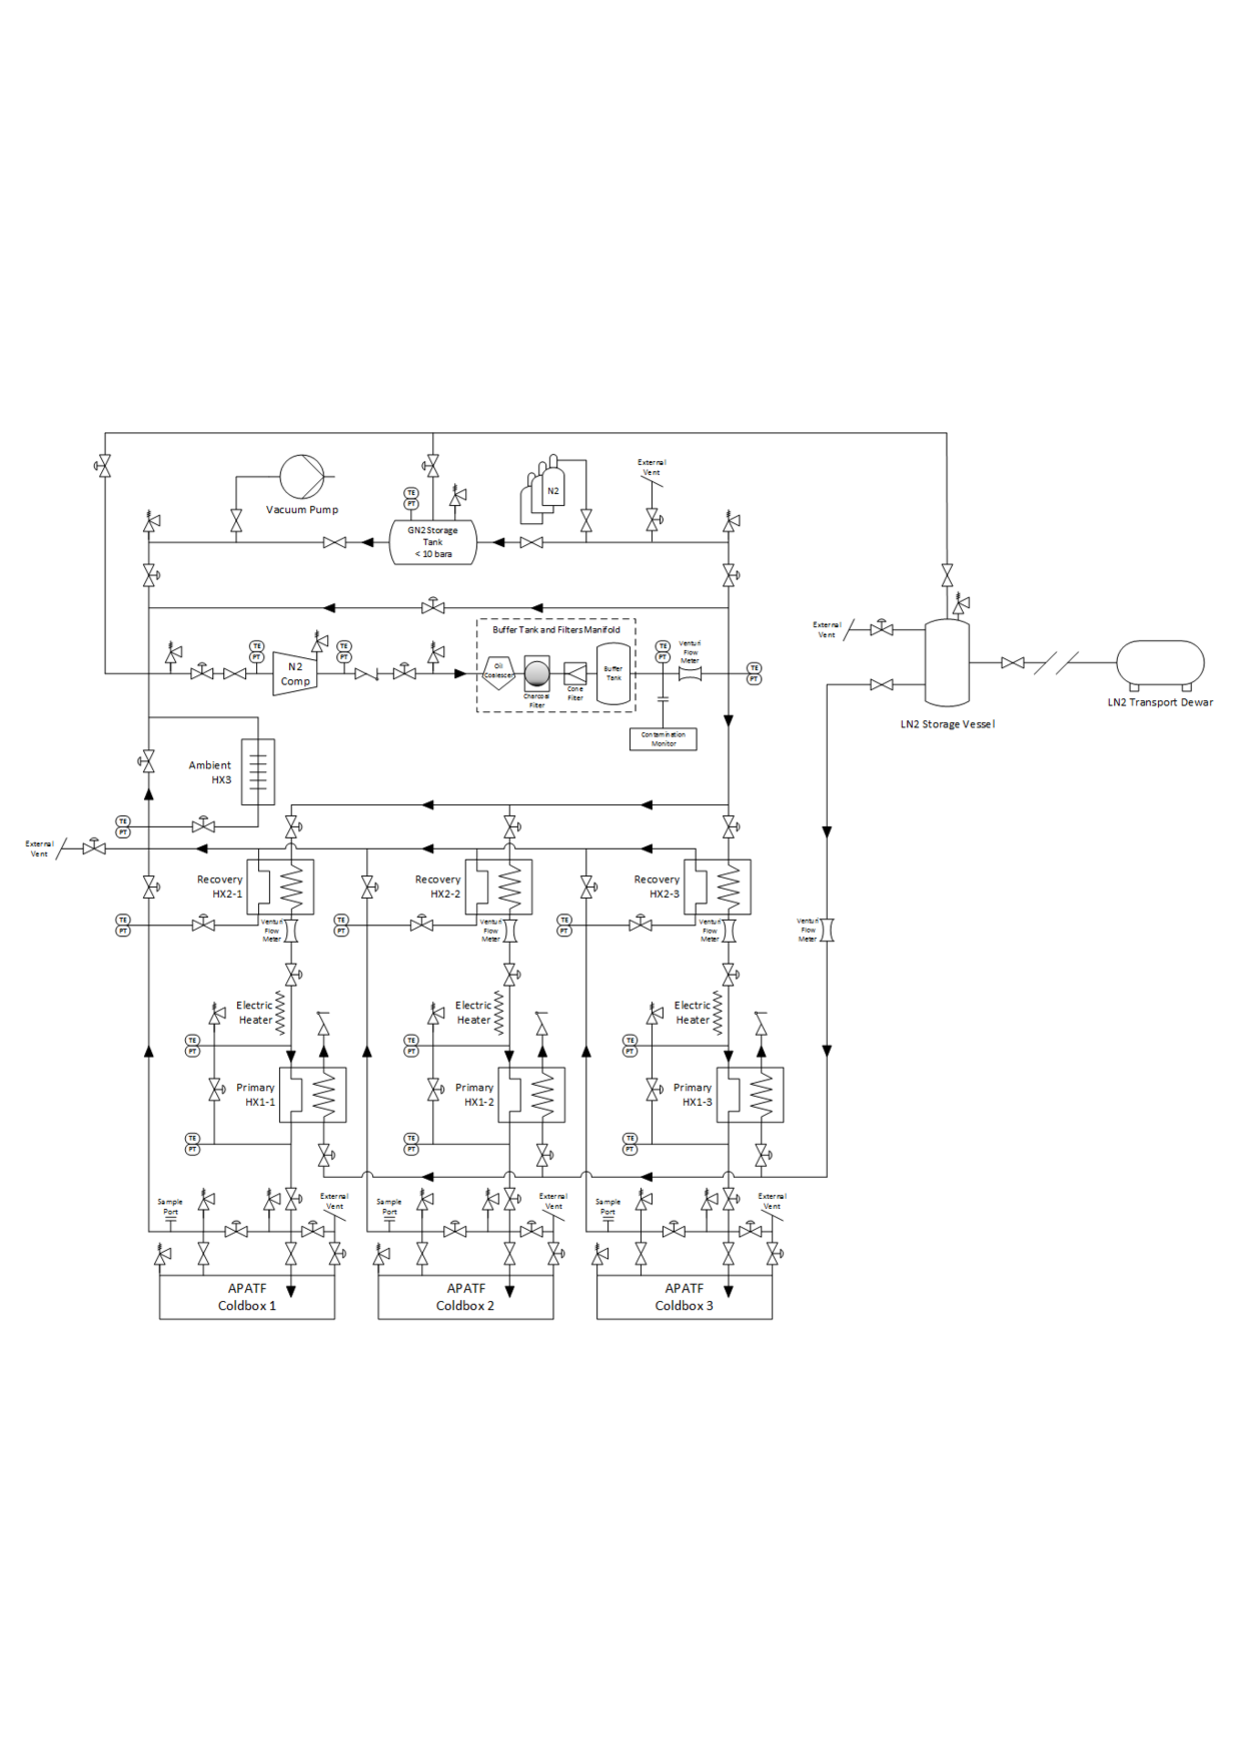
\includegraphics[width=.98\textwidth]{graphics/Cryo-cold-box-LN2.pdf}
\end{dunefigure}



%%%%%%%%%

% clear the figure buffer before starting the next section
\clearpage

%%%%%%%%%%%%%%%%%%%%%%%%%%%%
\subsection{Prototyping and Testing (QA/QC)}
\label{sec:fdsp-tc-infr-qaqc}

%The installation setup phase is where all of new equipment is installed underground. This represents a lot of new and unique work. While most of these installation procedures have already been tested during the trial assembly at Ash River, everything must be properly approved. The main \dword{apa} and \dword{cpa} towers will already be structurally approved, but load tests must be performed on all lifting fixtures, shuttle beams, crane tower connections, and \coldbox connections. 
Installing all this new equipment underground during the installation setup phase involves a lot of new techniques  and unique work. While most of the procedures will have been tested during the trial assembly at Ash River, everything must be properly approved. The main \dword{apa} and \dword{cpa} towers will already be structurally approved, but all lifting fixtures, shuttle beams, crane tower connections, and \coldbox connections must undergo load tests. 

%This is also when the \coldbox{}es and cryogenic system will be tested, so access to the cleanroom  may be restricted for several days for system checks.
The \coldbox{}es and cryogenic system will also be tested, so access to the cleanroom  may be restricted for several days for system checks.

%%%%%%%%%%%%%%%%%%%%%%%%%%%%
\subsection{Safety}
\label{sec:fdsp-tc-infr-safety}
%At this phase of construction of Detector 1, larger teams from the consortia, SDSD,  and contractors will need access to underground facilities at the same time \dword{lbnf} is completing the cold structure on Detector 1 and beginning the warm structure on Detector 2. Shift schedules now switch to 2 shifts/day because a maximum of 140 \dword{fte} can be underground at any given time.  Daily work meetings and safety coordination led by the shift supervisor at the start of each shift to coordinate work activities, hazard/mitigation reviews, and installation procedures are critical for a safe work environment. More details can be found in section 1.4.4 under the Installation \dword{esh} section. 
During this phase, as new equipment is being installed and tested, new employees and collaborators will be trained, and larger teams from the consortia, \dword{sdsd},  and contractors will need access to underground facilities.  This is at the same time that \dword{lbnf} is completing the cold structure on \dword{detmodule} \#1 and beginning the warm structure on  \dword{detmodule} \#2. Given the maximum of 140 \dword{fte} underground at any given time, we move to two shifts per day.  At the start of each shift, the shift supervisor will lead a work meeting to coordinate work activities, review hazards and mitigations, and review installation procedures to ensure a safe work environment. More details can be found in section 1.4.4 under the Installation \dword{esh} section. \fixme{anne to fix sectioning}

%The \dword{uit} will be extremely busy at this time. The crew sizes are increasing, so training new employees and consortia will be ongoing, and new equipment is being installed and tested. Proper documentation of structural calculations, assembly drawings, load tests, hazard analyses, and procedures will all have to be reviewed and approved before operational readiness is approved. This all helps prepare for a safe start to the underground installation. 
Proper documentation of structural calculations, assembly drawings, load tests, hazard analyses, and procedures will all have to be reviewed and approved before operational readiness is approved. \fixme{operational readiness? is this different from readiness to begin installation?} This all helps prepare for a safe start to the underground installation. 

%The \coldbox and cryogenic system is one of the few things in the installation process that will not be fully tested during any of the trial assembly work. While the design of the boxes are very similar to the what was done at CERN for \dword{protodune}, the major difference is the system requirement that it is safe for workers to be in the cleanroom during the cool down phase. Procedures for operating the \coldbox have not been defined, but a requirements document has been written.   
Unlike most items, the \coldbox and cryogenics system will not be fully tested during the trial assembly work. While the new \coldbox design is very similar to \dword{pdsp}'s, some new requirements are in effect. In particular, it is \fixme{now?} safe for workers to be in the cleanroom during the cool down phase. \fixme{it was permitted for protodune but is no longer safe, or it was not permitted earlier, but will be ok now?} Procedures for operating the \coldbox will be written following the established requirements. 

  
%%%%%%%%%%%%%%%%%%%%%%%%%%%%
\subsection{Costs, Schedule, and Risk Analysis}
\label{sec:fdsp-tc-infr-cost}

\fixme{Add costs when available}

{\bf Installation Setup Phase:} %This is a more difficult phase to schedule and may be adjusted often with multiple projects going forward at once. The \dword{cf} work is basically completed, which reduces the number of \dwords{fte} underground, allowing us to begin the installation infrastructure. We begin two 10 hour shifts per day as the work ramps up.  Once the cold cryostat is approximately six months into the installation schedule, floor space becomes available in the north cavern. The \coldbox construction must be started ASAP because the welding takes approximately six months. In parallel to this, the machine shop area can be set up and the bridge between the north and south sides of the cavern can be constructed.  Once the bridge is completed, work on the assembly crane, \dword{apa} cabling tower, \dword{apa} assembly tower, and \dword{cpa} assembly station can begin. 
    This is a more difficult phase to schedule and may require frequent adjustment, with multiple projects going forward at once. The \dword{cf} work is essentially completed by this point, which reduces the number of \dwords{fte} underground, allowing us to begin the installation infrastructure. 
    \fixme{Sort of a non sequitur. Reduced cf FTEs allows you to have more FTEs, but it's not clear that it's what allows you to begin the installation infra } We begin two ten-hour shifts per day as the work ramps up.  Once the  cryostat cold structure is approximately six months into the installation schedule, floor space becomes available in the north cavern. The \coldbox construction must begin immediately at this point because the welding takes approximately six months. In parallel, the machine shop area can be set up and the bridge between the north and south sides of the cavern can be constructed.  Once the bridge is completed, work on the assembly crane, \dword{apa} cabling tower, \dword{apa} assembly tower, and \dword{cpa} assembly station can begin. 
    
%Installation of the detector support system could begin during the final installation stages of the cryostat cold structure because they both require full height scaffolding for all the welding on the top of the cryostat. This was how the \dword{protodune} \dword{dss} was installed. The details have not yet been worked out with the contractor, so work may be done in stages. This requires a crew on top of the cryostat installing the \dword{dss} support feedhroughs from the top of the cryostat as shown in Figure \ref{fig:install-dss-feedthru}. 
Installation of the \dword{dss} could begin during the final installation stages of the cryostat cold structure because they both require full-height scaffolding for the welding on the top of the cryostat. The \dword{protodune} \dword{dss} was installed this way. This requires a crew on top of the cryostat installing the \dword{dss} support feedhroughs from the top, as shown in Figure~\ref{fig:install-dss-feedthru}.  The details have not yet been worked out with the contractor, so work may be done in stages. 

A detailed schedule of the installation infrastructure time period is shown in Figure~\ref{fig:Installation_Infrastructure_Schedule}.
    
\begin{dunefigure}[Schedule for the infrastructure installation]
{fig:Installation_Infrastructure_Schedule}
    {Schedule for the infrastructure installation}
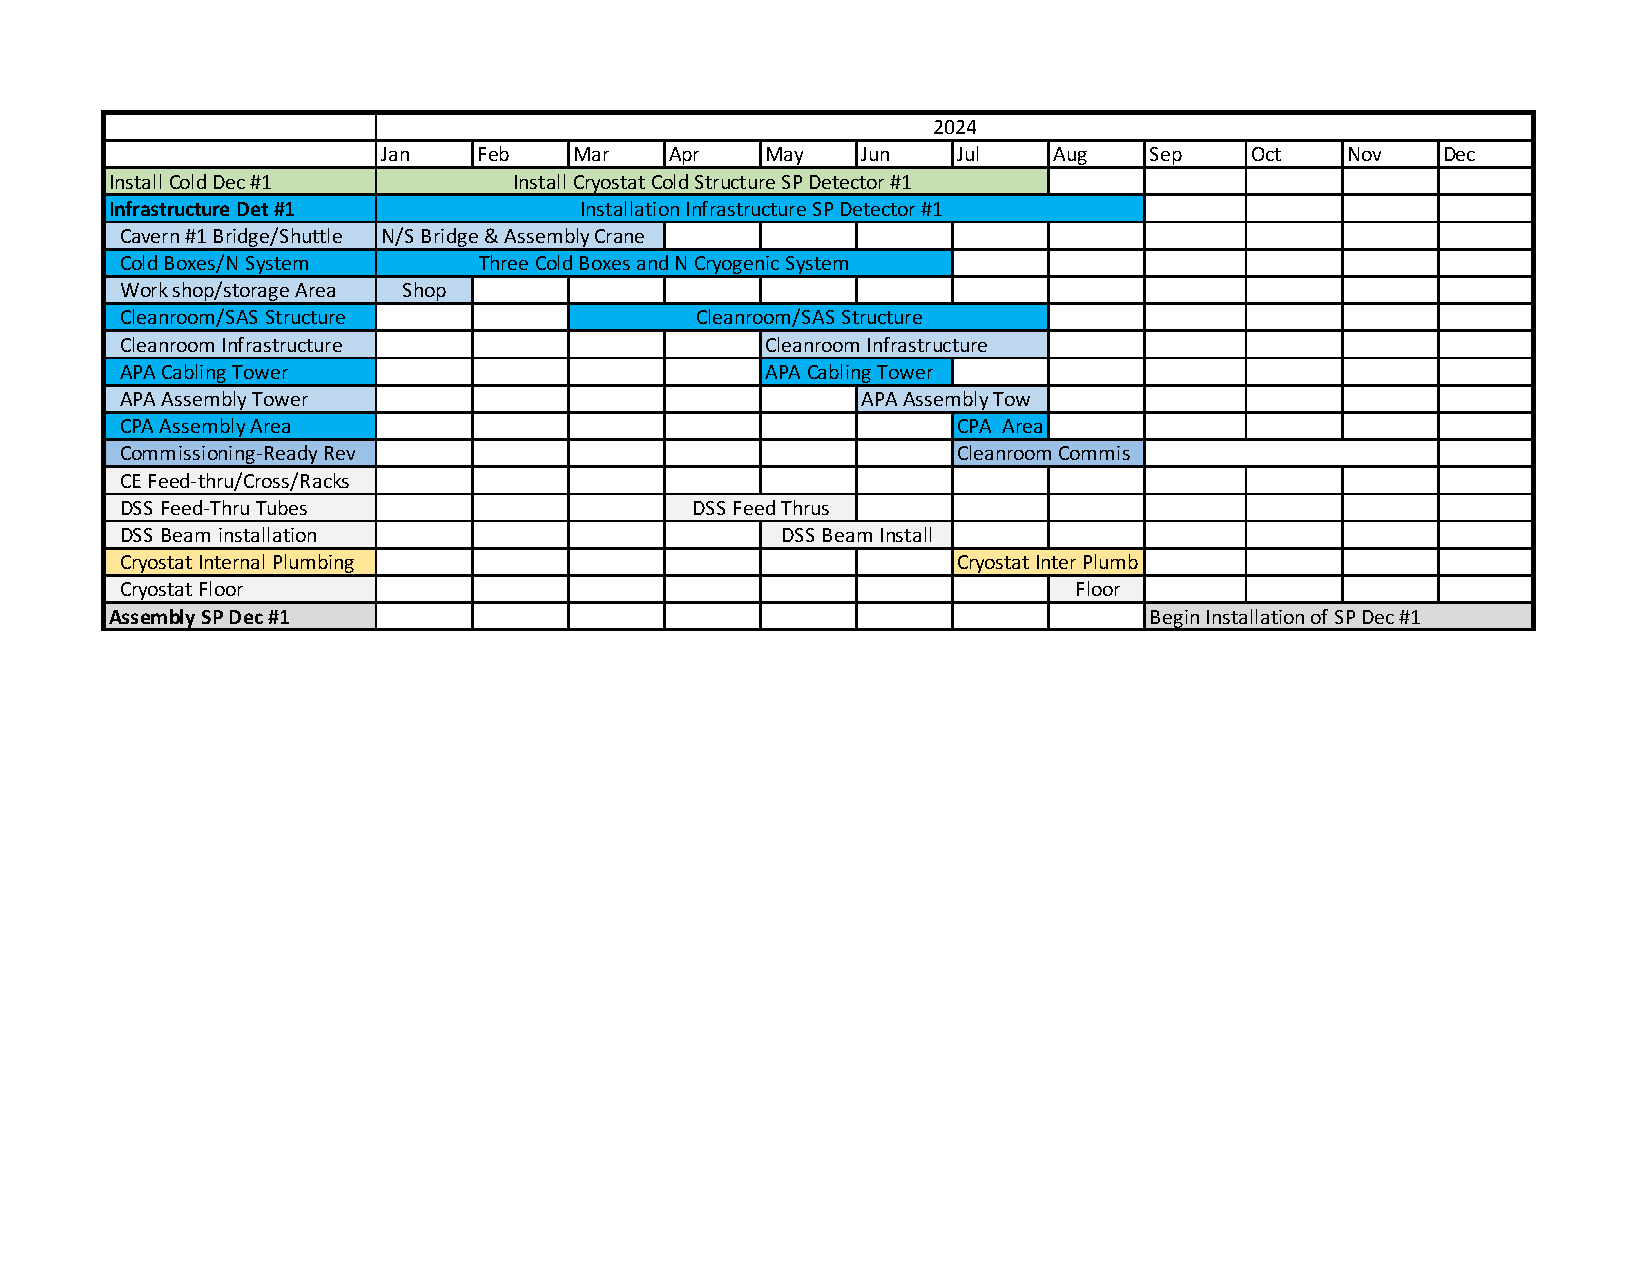
\includegraphics[width=0.98\textwidth]
{Installation_Infrastructure_Schedule} 
\end{dunefigure}

\fixme{A graphical representation of the schedule is used since it is critical to convey the time sequencing and how the work is overlapping. Jim }

% clear the figure buffer before starting the next section
\clearpage
